\section{Evaluation Results} \label{sec:appendix-quantitative}

\subsection{Main Results}
Table \ref{tab:benchmark-results} shows the pass@1 and pass@5 results of all evaluated models on \benchmark, and Fig. \ref{fig:main-results-all-appendix} shows them in box-plot form.

\begin{table}[htbp]
    \centering
    \caption{Results of all models on \benchmark}
    \begin{tabular}{cccccc}
        \toprule
        \multirow{2}{*}{\textbf{Model}} & \multirow{2}{*}{\textbf{Size}} & \multicolumn{2}{c}{\textbf{Input Prediction}} & \multicolumn{2}{c}{\textbf{Output Prediction}} \\
        \cmidrule(lr){3-4} \cmidrule(lr){5-6}
        & & \textbf{Pass@1} & \textbf{Pass@5} & \textbf{Pass@1} & \textbf{Pass@5} \\
	\midrule
	\multirow{3}{*}{CodeLlama}
	& 7B & 36.6\% & 55.2\% & 36.4\% & 49.6\% \\
	& 13B & 39.0\% & 58.2\% & 38.4\% & 53.2\% \\
	& 34B & 46.5\% & 64.7\% & 41.1\% & 56.1\% \\
	\midrule
	\multirow{3}{*}{CodeLlama Python}
	& 7B & 36.3\% & 56.0\% & 36.4\% & 49.7\% \\
	& 13B & 40.5\% & 58.0\% & 37.8\% & 50.8\% \\
	& 34B & 41.5\% & 59.2\% & 40.7\% & 53.7\% \\
	\midrule
	\multirow{2}{*}{StarCoder-Base}
	& 7B & 30.0\% & 48.9\% & 31.1\% & 43.8\% \\
	& 15.5B & 31.6\% & 49.5\% & 33.3\% & 47.7\% \\
	\midrule
	\multirow{2}{*}{WizardCoder}
	& 13B & 39.2\% & 54.8\% & 37.9\% & 51.6\% \\
	& 34B & 42.8\% & 57.3\% & 41.2\% & 52.2\% \\
	\midrule
	Phi-1
	& 1.3B & 13.9\% & 22.6\% & 23.3\% & 34.0\% \\
	\midrule
	Phi-1.5
	& 1.3B & 24.1\% & 38.9\% & 27.1\% & 39.4\% \\
	\midrule
	Phind v2
	& 34B & 47.9\% & 64.9\% & 38.3\% & 49.2\% \\
	\midrule
	\multirow{2}{*}{Deepseek Coder-Base}
	& 6.7B & 41.1\% & 61.7\% & 39.8\% & 53.9\% \\
	& 33B & 46.6\% & 65.1\% & 43.6\% & 57.6\% \\
	\midrule
	\multirow{2}{*}{Deepseek Coder-Instruct}
	& 6.7B & 36.6\% & 54.4\% & 41.0\% & 52.5\% \\
	& 33B & 47.4\% & 64.2\% & 44.0\% & 58.0\% \\
	\midrule
	Mistral
	& 7B & 36.0\% & 54.2\% & 31.7\% & 45.2\% \\
	\midrule
	GPT-3.5
	& - & 49.2\% & 66.5\% & 50.0\% & 60.1\% \\
	\midrule
	GPT-4
	& - & 67.1\% & 76.8\% & 63.4\% & 68.7\% \\
    \bottomrule
    \end{tabular}
    \label{tab:benchmark-results}
\end{table}


% \begin{figure}[H]
%      \centering
%      \begin{subfigure}[b]{0.49\textwidth}
%          \centering
%          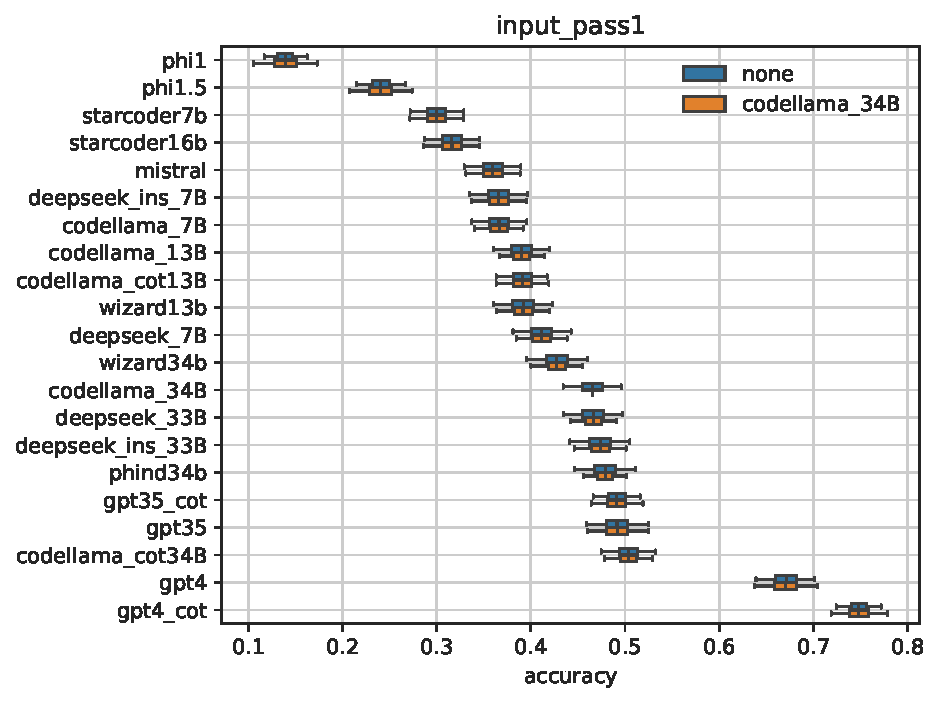
\includegraphics[width=\textwidth]{figs/main_results/main_box_input_pass1.pdf}
%          \caption{Performance, pass@1 (Input)}
%          \label{fig:main-results-pass1-input}
%      \end{subfigure}
%      \hfill
%      \begin{subfigure}[b]{0.49\textwidth}
%          \centering
%          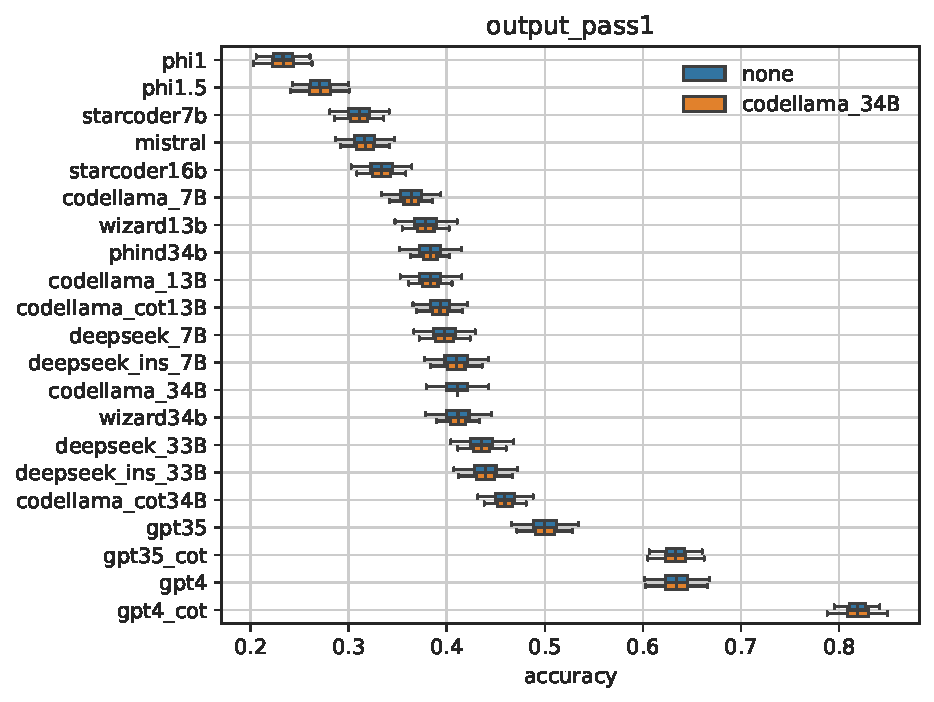
\includegraphics[width=\textwidth]{figs/main_results/main_box_output_pass1.pdf}
%          \caption{Performance, pass@1 (Output)}
%          \label{fig:main-results-pass1-output}
%      \end{subfigure}
%      \caption{Boxes show (25, 75) percentiles and whiskers show (2.5, 97.5) independently and when all models are compared against \codellamalarge as the baseline where the difference between more pairs are significant. }
%      \label{fig:baseline_results}
% \end{figure}

\begin{figure}[H]
     \centering
     \begin{subfigure}[b]{0.49\textwidth}
         \centering
         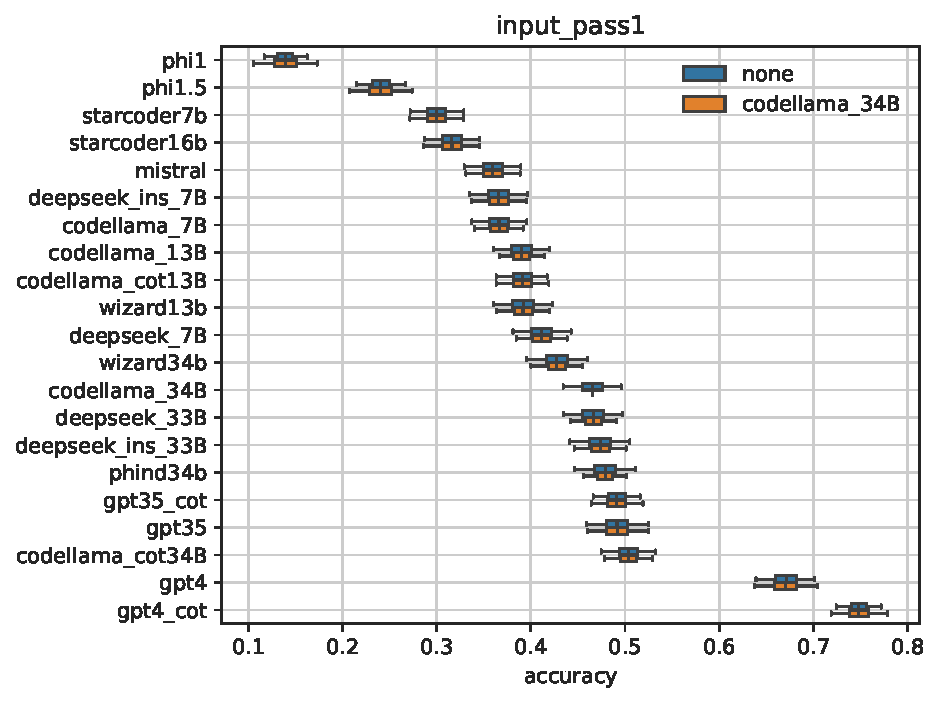
\includegraphics[scale=0.4]{figs/main_results/main_box_input_pass1.pdf}
         \caption{Main Results, pass@1 (Input)}
         \label{fig:main-results-pass1-input-appendix}
     \end{subfigure}
     \hfill
     \begin{subfigure}[b]{0.49\textwidth}
         \centering
         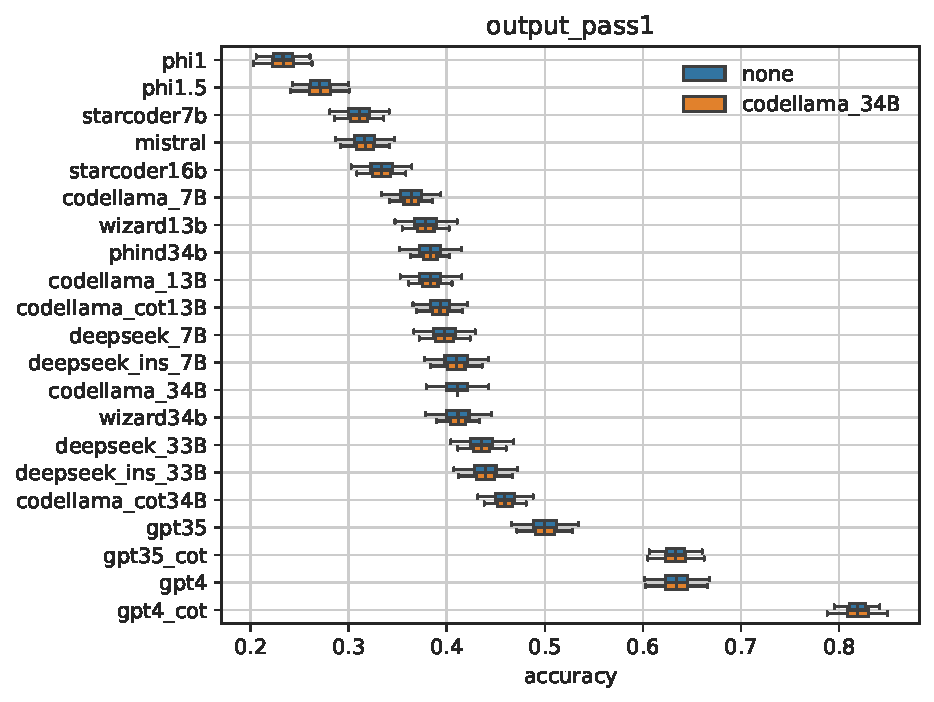
\includegraphics[scale=0.4]{figs/main_results/main_box_output_pass1.pdf}
         \caption{Main Results, pass@1 (Output)}
         \label{fig:main-results-pass1-output-appendix}
     \end{subfigure}
     \newline
     \newline
     \begin{subfigure}[b]{0.49\textwidth}
         \centering
         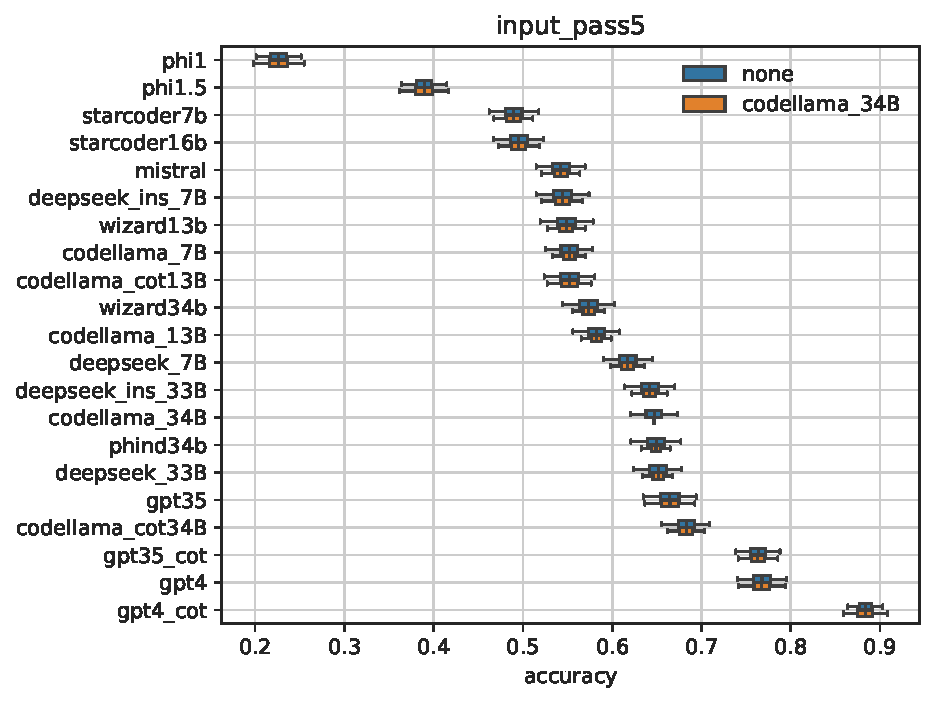
\includegraphics[scale=0.4]{figs/main_results/main_box_input_pass5.pdf}
         \caption{Main Results, pass@5 (Input)}
         \label{fig:main-results-pass5-input-appendix}
     \end{subfigure}
     \hfill
     \begin{subfigure}[b]{0.49\textwidth}
         \centering
         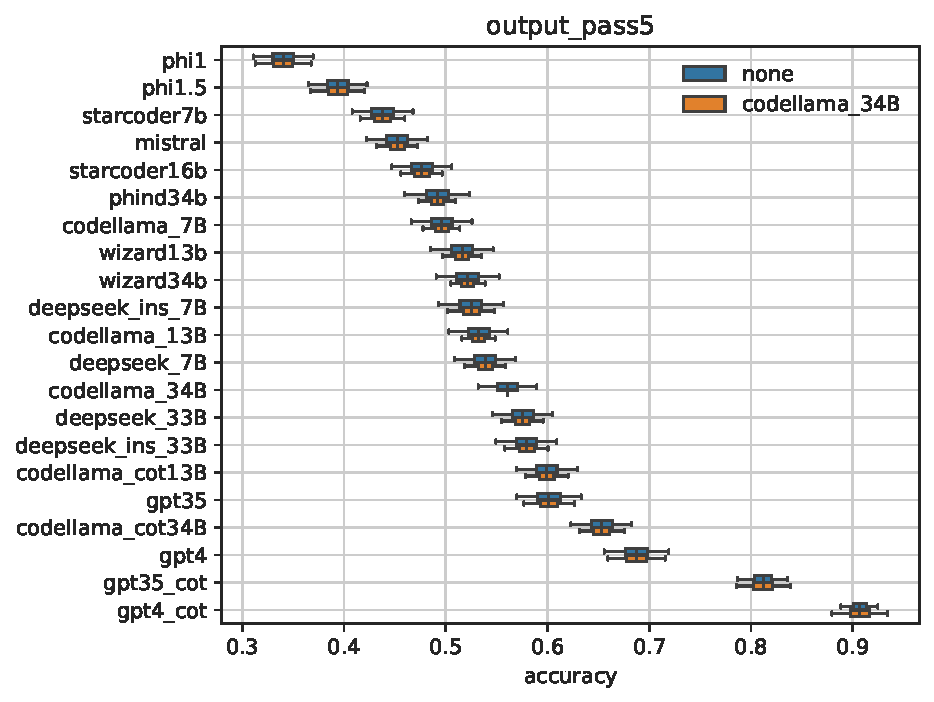
\includegraphics[scale=0.4]{figs/main_results/main_box_output_pass5.pdf}
         \caption{Main Results, pass@5 (Output)}
         \label{fig:main-results-pass5-output-appendix}
     \end{subfigure}
     \caption{Main Results with confidence intervals compared to codellama\_34B.}
     \label{fig:main-results-all-appendix}
\end{figure}

\subsection{Additional Results on Impact of CoT} \label{subsec:appendix-cot}
Table \ref{tab:benchmark-results-cot} shows the results of including CoT on Code Llama 13B, 34B, GPT-3.5, and GPT-4.

\begin{table}[h]
    \centering
    \caption{Impact of CoT on \benchmark}
    \begin{tabular}{cccccc}
        \toprule
        \multirow{2}{*}{\textbf{Model}} & \multirow{2}{*}{\textbf{CoT}} & \multicolumn{2}{c}{\textbf{Input Prediction}} & \multicolumn{2}{c}{\textbf{Output Prediction}} \\
        \cmidrule(lr){3-4} \cmidrule(lr){5-6}
        & & \textbf{Pass@1} & \textbf{Pass@5} & \textbf{Pass@1} & \textbf{Pass@5} \\
	\midrule
	\multirow{3}{*}{Code Llama 13B}
	& \xmark & 39.0\% & 58.2\% & 38.4\% & 53.2\% \\
	& \cmark & 39.1\% & 55.2\% & 39.3\% & 59.9\% \\
	& - & \green{+0.1\%} & \red{-3.0\%} & \green{+0.9\%} & \green{+6.7\%} \\
	\midrule
	\multirow{3}{*}{Code Llama 34B}
	& \xmark & 46.5\% & 64.7\% & 41.1\% & 56.1\% \\
	& \cmark & 50.4\% & 68.3\% & 46.0\% & 65.3\% \\
	& - & \green{+3.9\%} & \green{+3.6\%} & \green{+4.9\%} & \green{+9.2\%} \\
	\midrule
	\multirow{3}{*}{GPT-3.5}
	& \xmark & 49.2\% & 66.5\% & 50.0\% & 60.1\% \\
	& \cmark & 49.1\% & 76.3\% & 63.3\% & 81.2\% \\
	& - & \red{-0.1\%} & \green{+9.8\%} & \green{+13.3\%} & \green{+21.1\%} \\
	\midrule
	\multirow{3}{*}{GPT-4}
	& \xmark & 67.1\% & 76.8\% & 63.4\% & 68.7\% \\
	& \cmark & 74.8\% & 88.4\% & 81.9\% & 90.7\% \\
	& - & \green{+7.7\%} & \green{+11.6\%} & \green{+18.5\%} & \green{+22.0\%} \\
        \bottomrule
    \end{tabular}
    \label{tab:benchmark-results-cot}
\end{table}


\textbf{Sample-wide improvements from CoT}: In Fig. \ref{fig:difference-hist-all}, we show a histogram of how much CoT improves the pass@1 score of each sample (negative values means that CoT decreased the accuracy). We observe that CoT leads to little improvement for the majority of samples, this effect is partly due to samples already having high pass@1 scores. As evidenced by Fig. \ref{fig:difference-hist-all-gpt4}, we see that CoT is much more effective for GPT-4 output prediction compared to both GPT-4 input prediction and other models. For the other models, however, we observe a large proportion of samples for which CoT actually decreases the pass@1. 

\begin{figure}[H]
     \centering
     \begin{subfigure}[t]{0.49\textwidth}
         \centering
         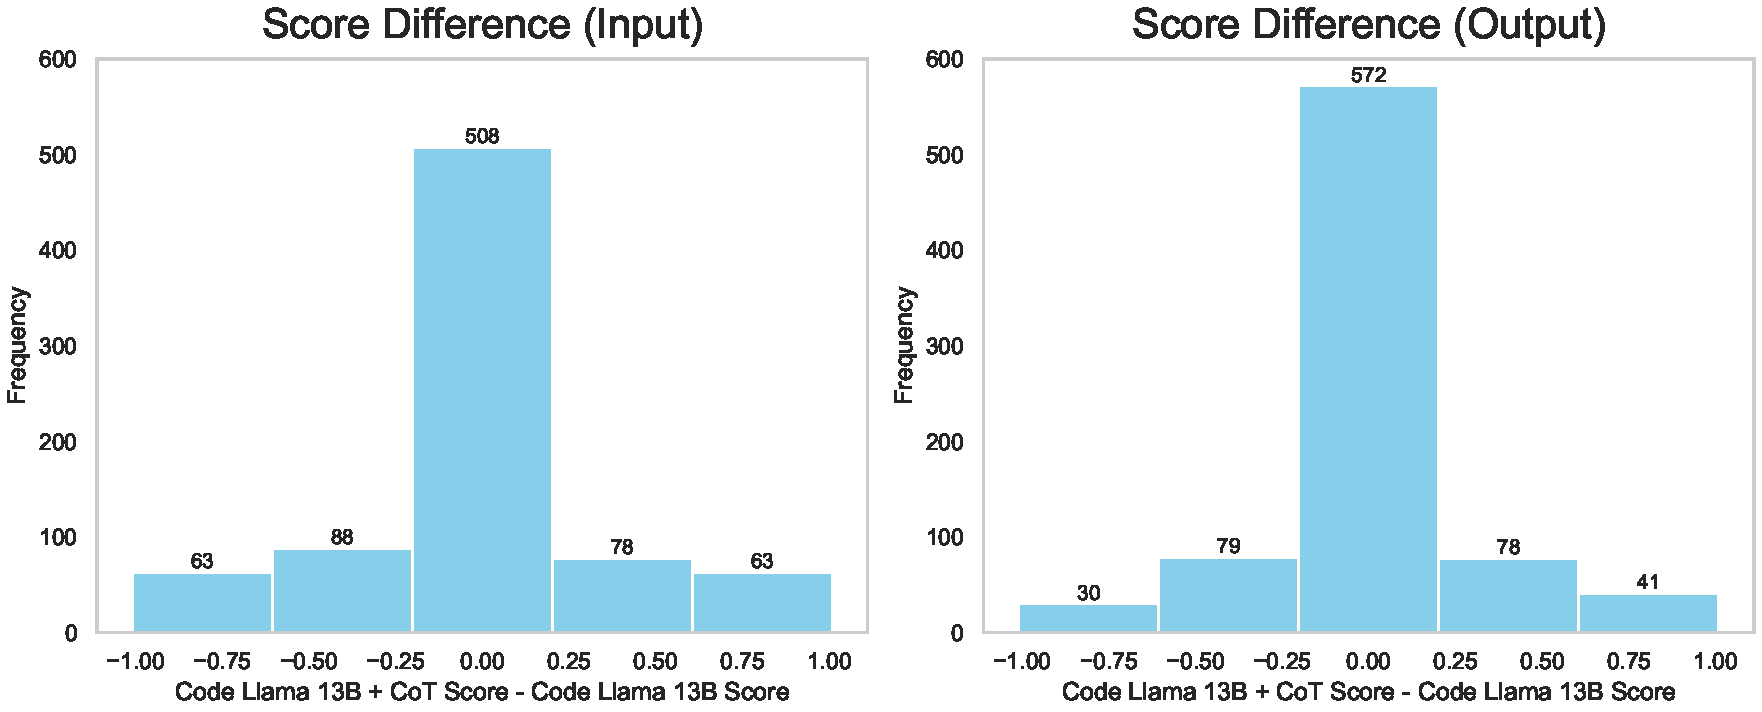
\includegraphics[width=\textwidth]{figs/confusion_cot/difference_histogram_codellama_13B_codellama_cot13B.pdf}
         \caption{Code Llama 13B}
     \end{subfigure}%
     \hfill
     \begin{subfigure}[t]{0.49\textwidth}
         \centering
         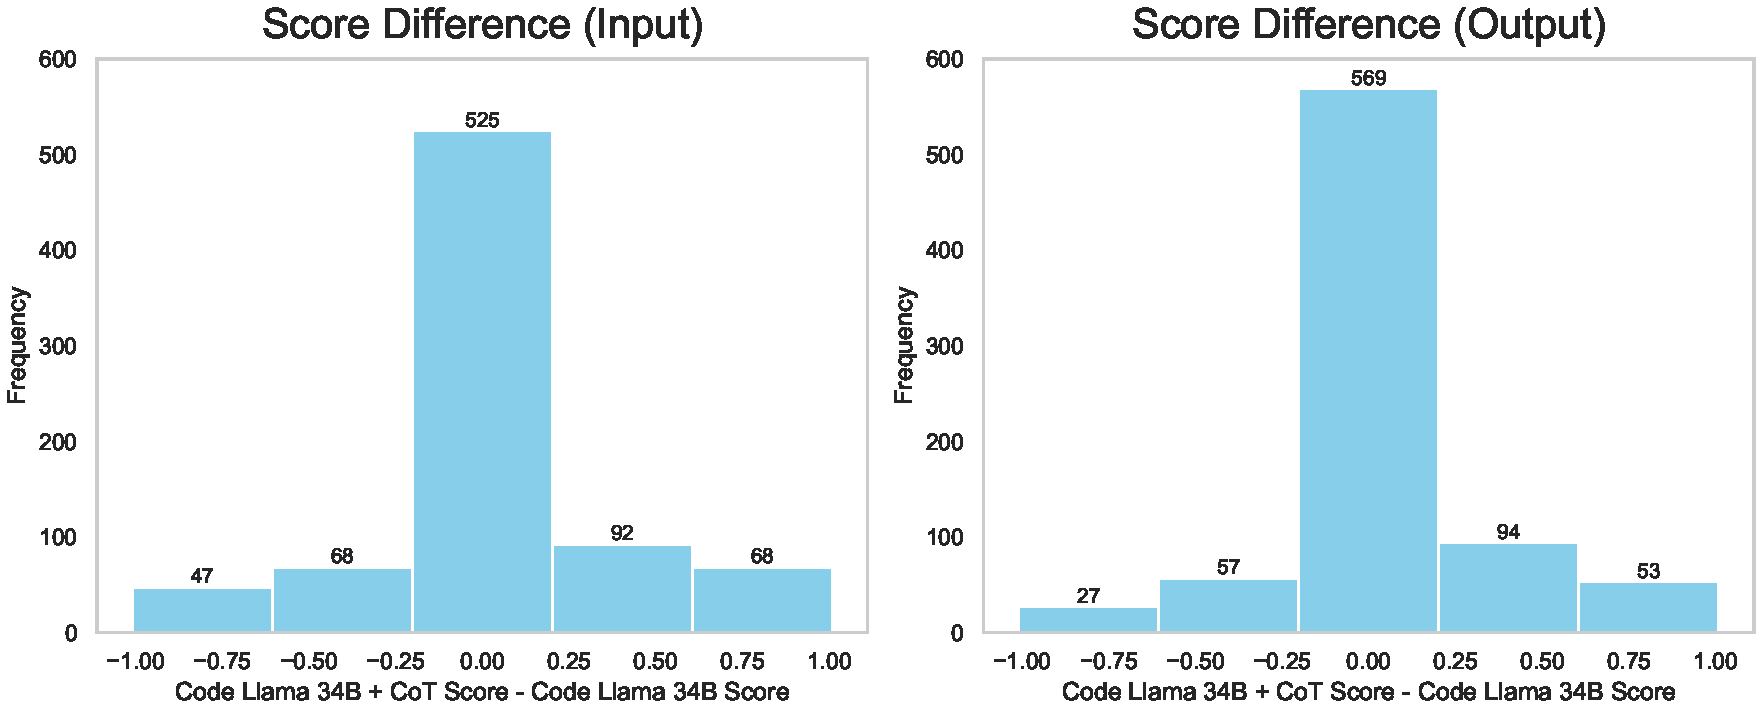
\includegraphics[width=\textwidth]{figs/confusion_cot/difference_histogram_codellama_30B_codellama_cot30B.pdf}
         \caption{Code Llama 34B}
     \end{subfigure}
     \newline
     \newline
     \newline
     \begin{subfigure}[t]{0.49\textwidth}
         \centering
         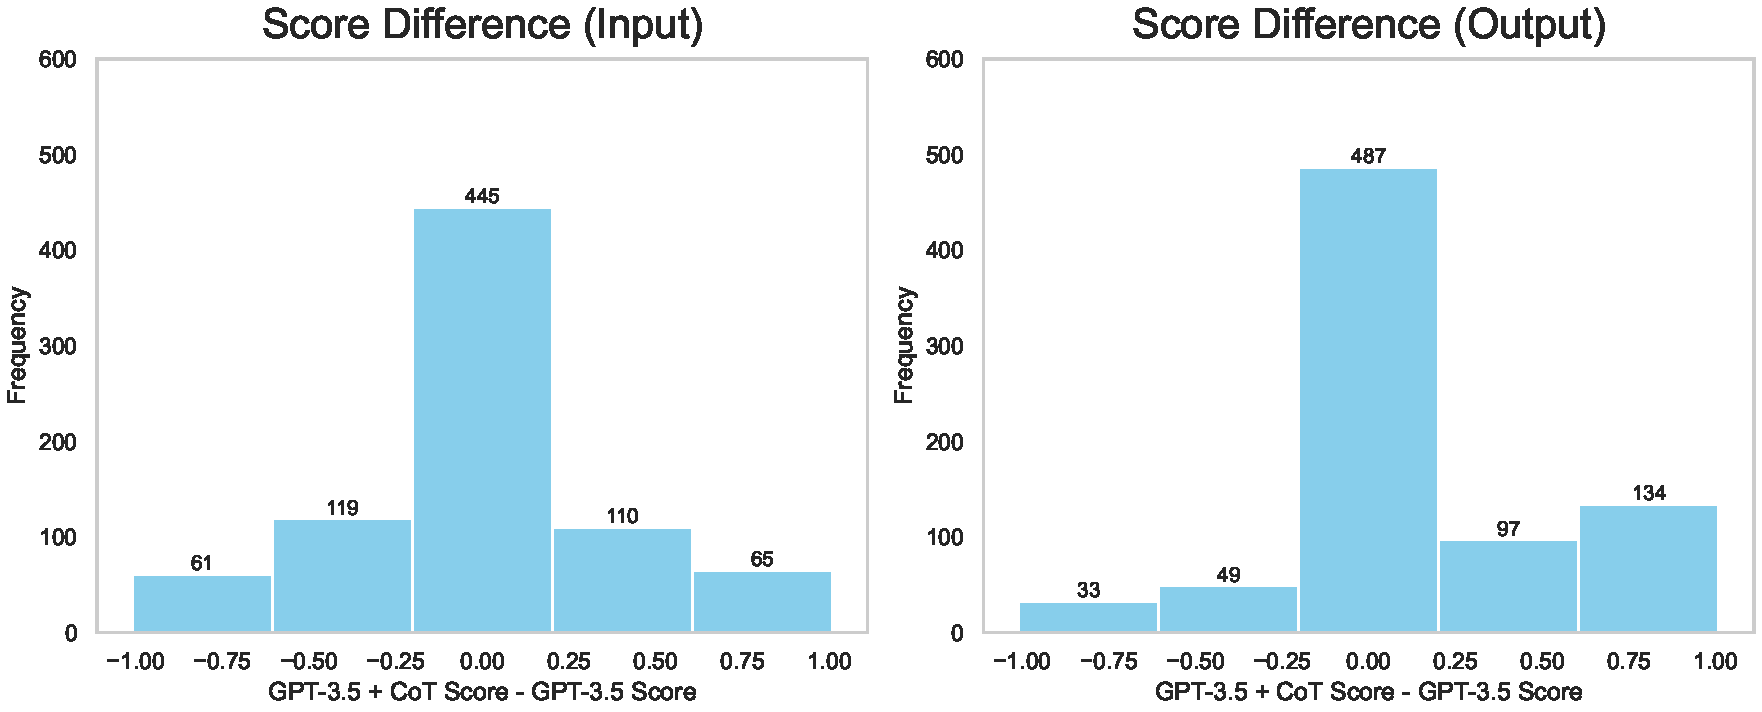
\includegraphics[width=\textwidth]{figs/confusion_cot/difference_histogram_gpt35_gpt35_cot.pdf}
         \caption{GPT-3.5}
     \end{subfigure}%
     \hfill
     \begin{subfigure}[t]{0.49\textwidth}
         \centering
         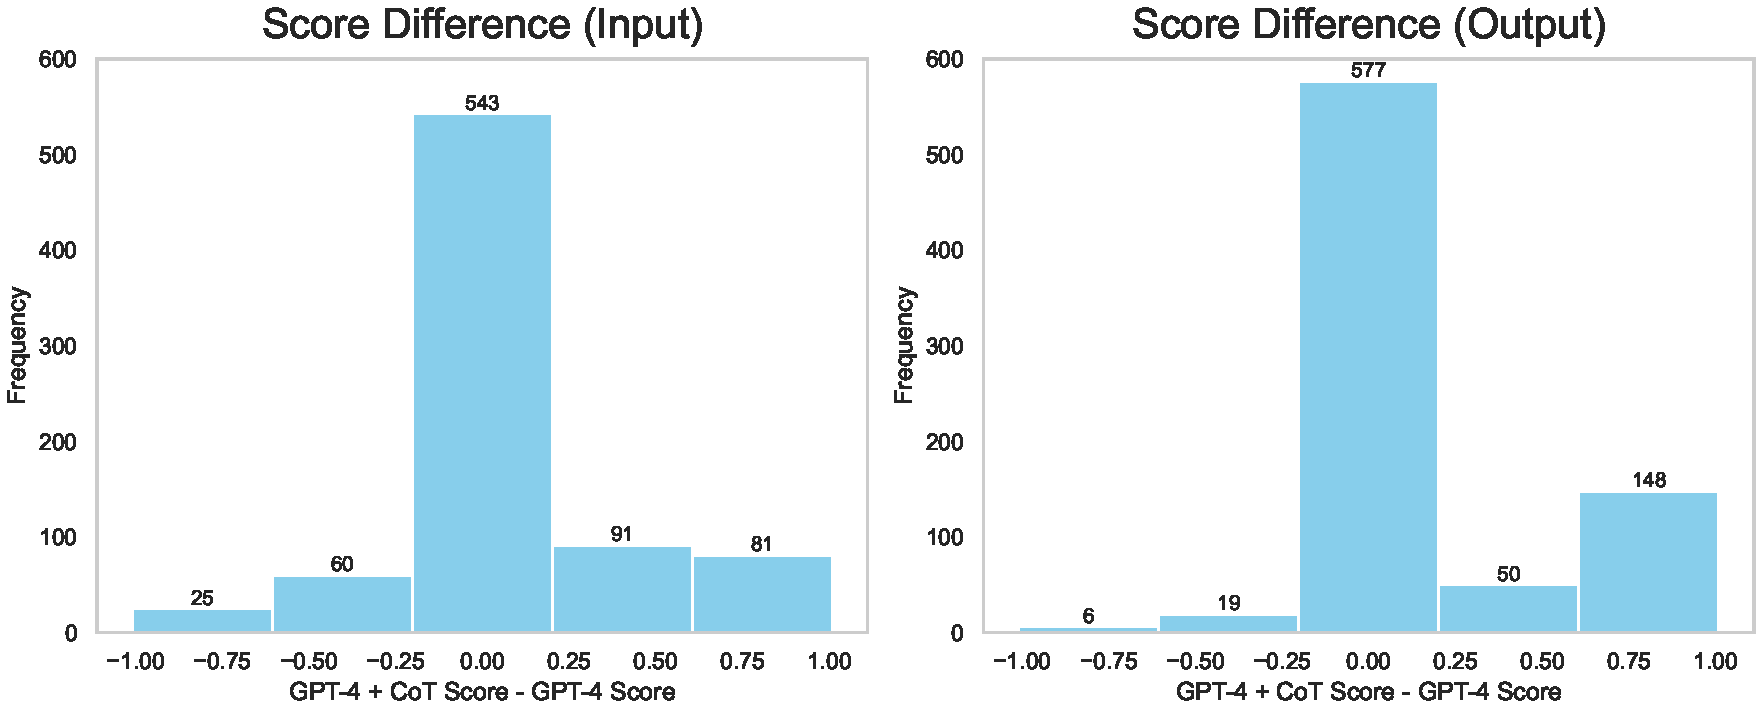
\includegraphics[width=\textwidth]{figs/confusion_cot/difference_histogram_gpt4_gpt4_cot.pdf}
         \caption{GPT-4}
         \label{fig:difference-hist-all-gpt4}
     \end{subfigure}
     \caption{Histogram of Score Differences between CoT and Original $(T=0.2)$}
     \label{fig:difference-hist-all}
\end{figure}

In Fig. \ref{fig:confusion-cot-all-granular}, we show a more granular perspective of Fig. \ref{fig:confusion-cot-all}, which again highlights that CoT often decreases the pass@1 score of many samples. Again, we observe a stark difference between the impact of CoT on GPT-4 and other models.

\begin{figure}[H]
     \centering
     \begin{subfigure}[t]{0.49\textwidth}
         \centering
         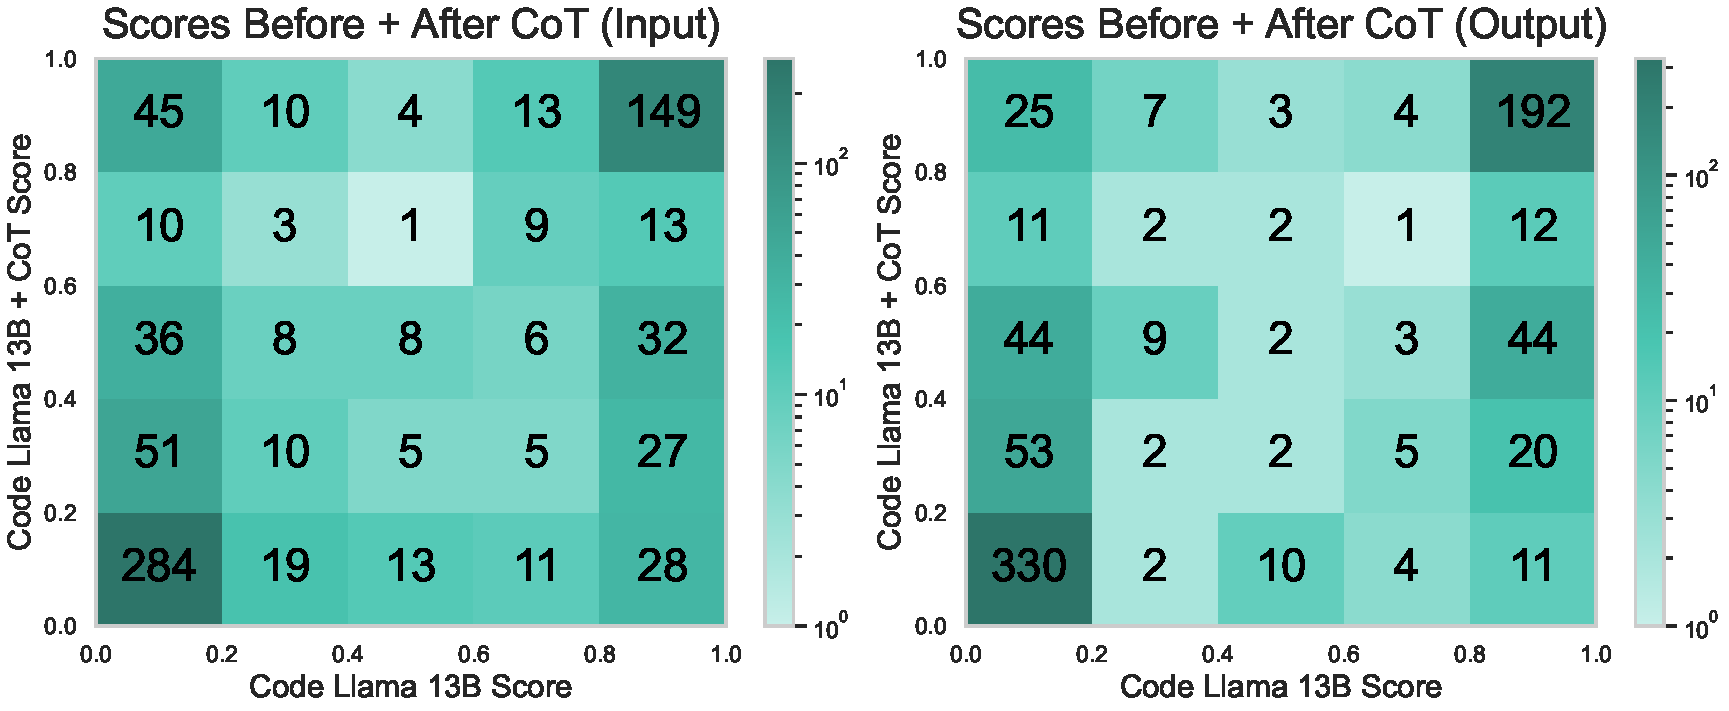
\includegraphics[width=\textwidth]{figs/confusion_cot/cot_confusion_granular_codellama_13B.pdf}
         \caption{Code Llama 13B}
     \end{subfigure}%
     \hfill
     \begin{subfigure}[t]{0.49\textwidth}
         \centering
         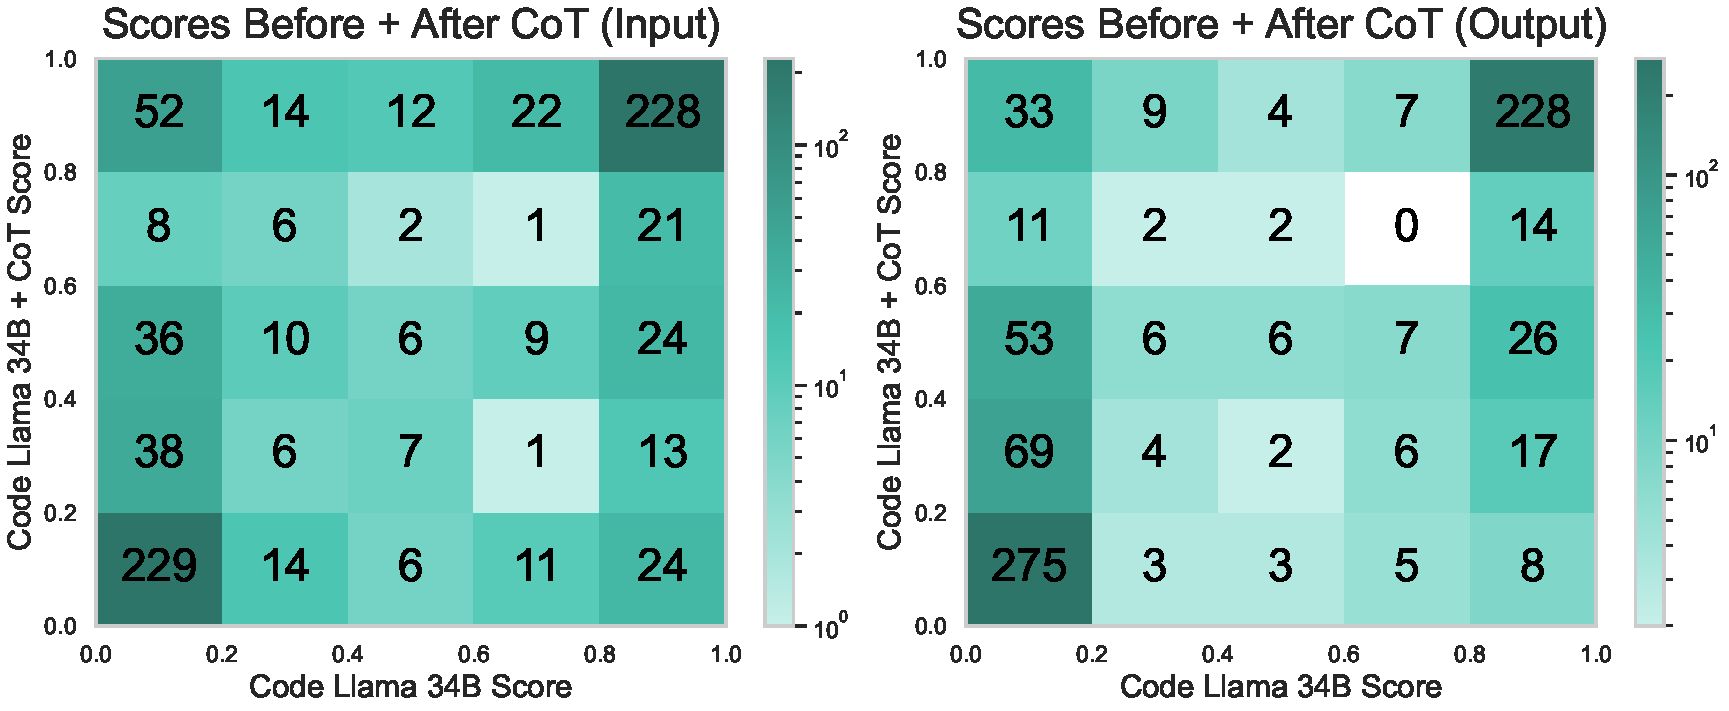
\includegraphics[width=\textwidth]{figs/confusion_cot/cot_confusion_granular_codellama_30B.pdf}
         \caption{Code Llama 34B}
     \end{subfigure}
     \newline
     \newline
     \newline
     \begin{subfigure}[t]{0.49\textwidth}
         \centering
         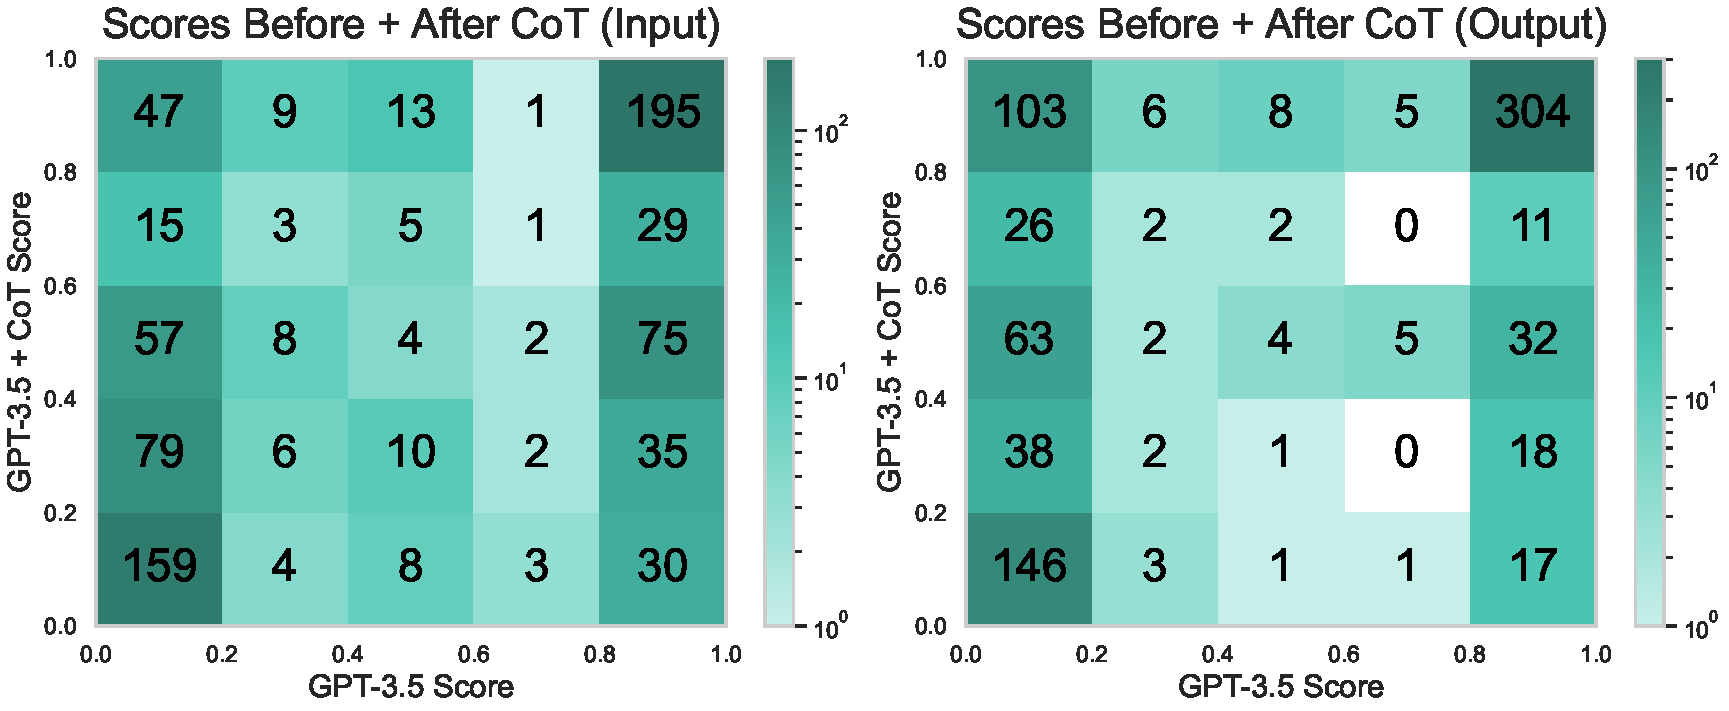
\includegraphics[width=\textwidth]{figs/confusion_cot/cot_confusion_granular_gpt35.pdf}
         \caption{GPT-3.5}
     \end{subfigure}%
     \hfill
     \begin{subfigure}[t]{0.49\textwidth}
         \centering
         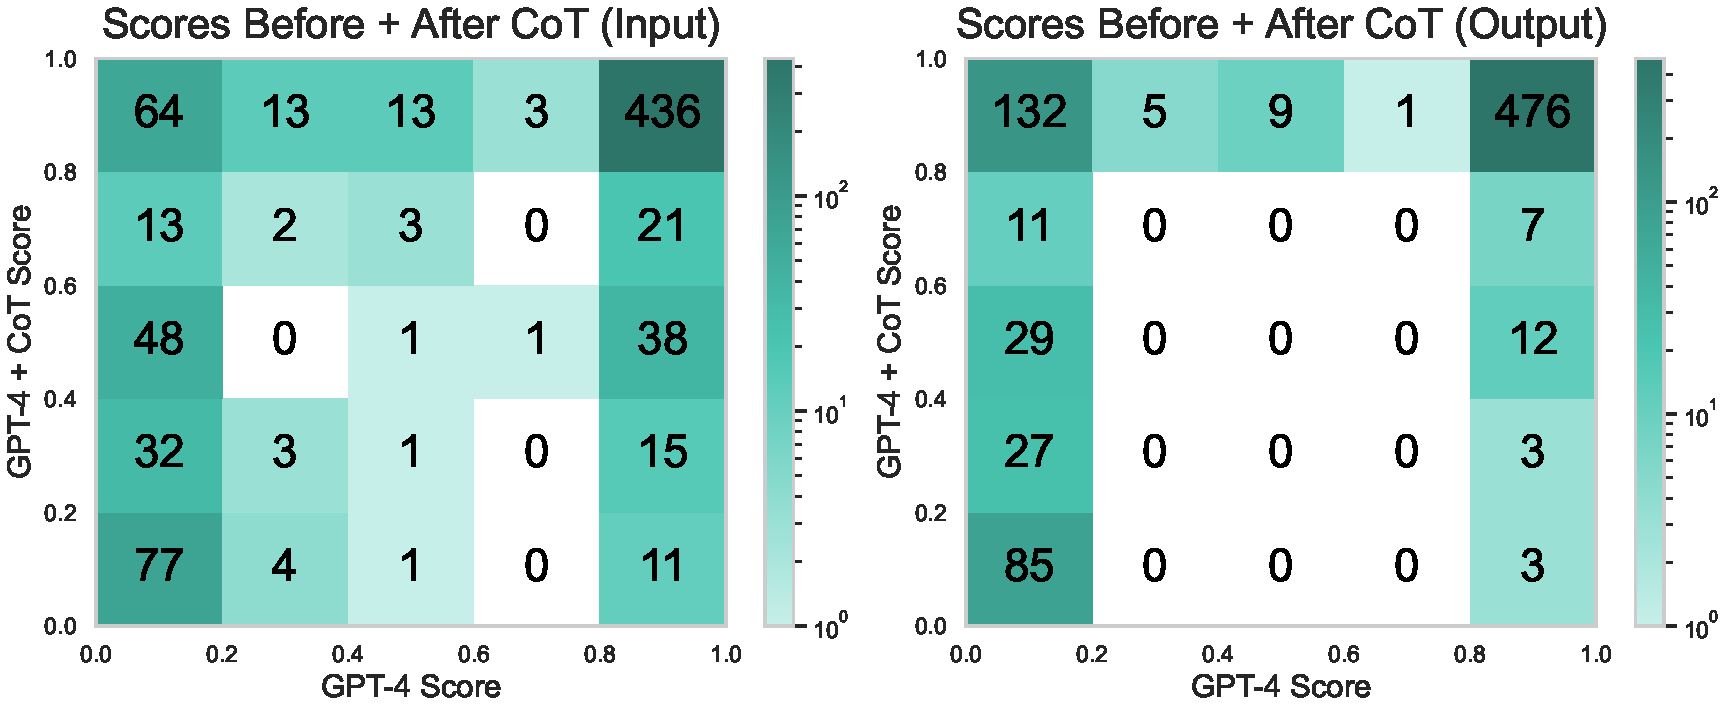
\includegraphics[width=\textwidth]{figs/confusion_cot/cot_confusion_granular_gpt4.pdf}
         \caption{GPT-4}
     \end{subfigure}
     \caption{Confusion Matrix of Direct Prediction vs. CoT Prediction $(T=0.2)$, Granular Version}
     \label{fig:confusion-cot-all-granular}
\end{figure}

\textbf{Qualitative example of CoT harming performance}: Finally, we show one example of input prediction and one example of output prediction where GPT-4 succeeds without CoT and fails with CoT.
\begin{lstlisting}
# Output Prediction
def f(phone_number):
    while phone_number.find('77777') != -1:
        phone_number = phone_number.replace('77777', 'seg', 1)
    return phone_number
assert f('7747777722') == '774seg22'

# GPT-4 CoT says that '77777' is not in '7747777722', returning '7747777722'
\end{lstlisting}

\begin{lstlisting}
# Input Prediction
def f(mylist):
    revl = mylist[:]
    revl.reverse()
    mylist.sort(reverse=True)
    return mylist == revl
assert f([5, 8]) == True

# GPT-4 CoT correctly says that "we need to provide a list that remains the same when sorted in descending order and when reversed," but then says the list should already be sorted in descending order, returning f([5, 4, 3, 2, 1]).
\end{lstlisting}

\textbf{Correlations between failures of different models}: Fig.~\ref{fig:error_prob-input-output} shows $P(Y \mid X=0) / P(Y)$, the accuracy of model $Y$ given that model $X$ fails completely relative to the original accuracy of model $Y$. Although what is hard for a better model tend to be hard for worse models on average, worse models succeeded on some examples where the better models fail completely, showing idiosyncrasies in failures even for the best \textsc{GPT-4 CoT} model.
\begin{figure}[H]
     \centering
     \begin{subfigure}[b]{0.49\textwidth}
         \centering
         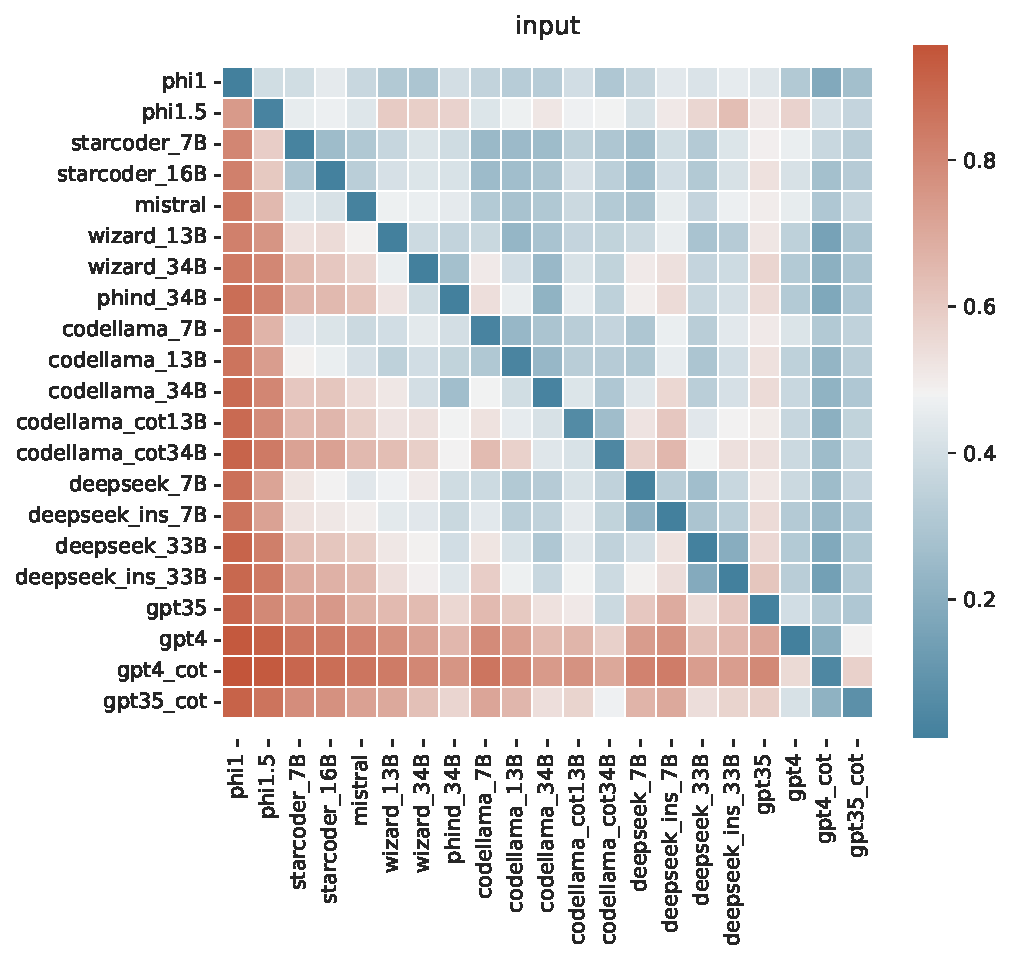
\includegraphics[width=1\textwidth]{figs/error_prob_input_heatmap.pdf}
     \end{subfigure}
     \hfill
     \begin{subfigure}[b]{0.49\textwidth}
         \centering
         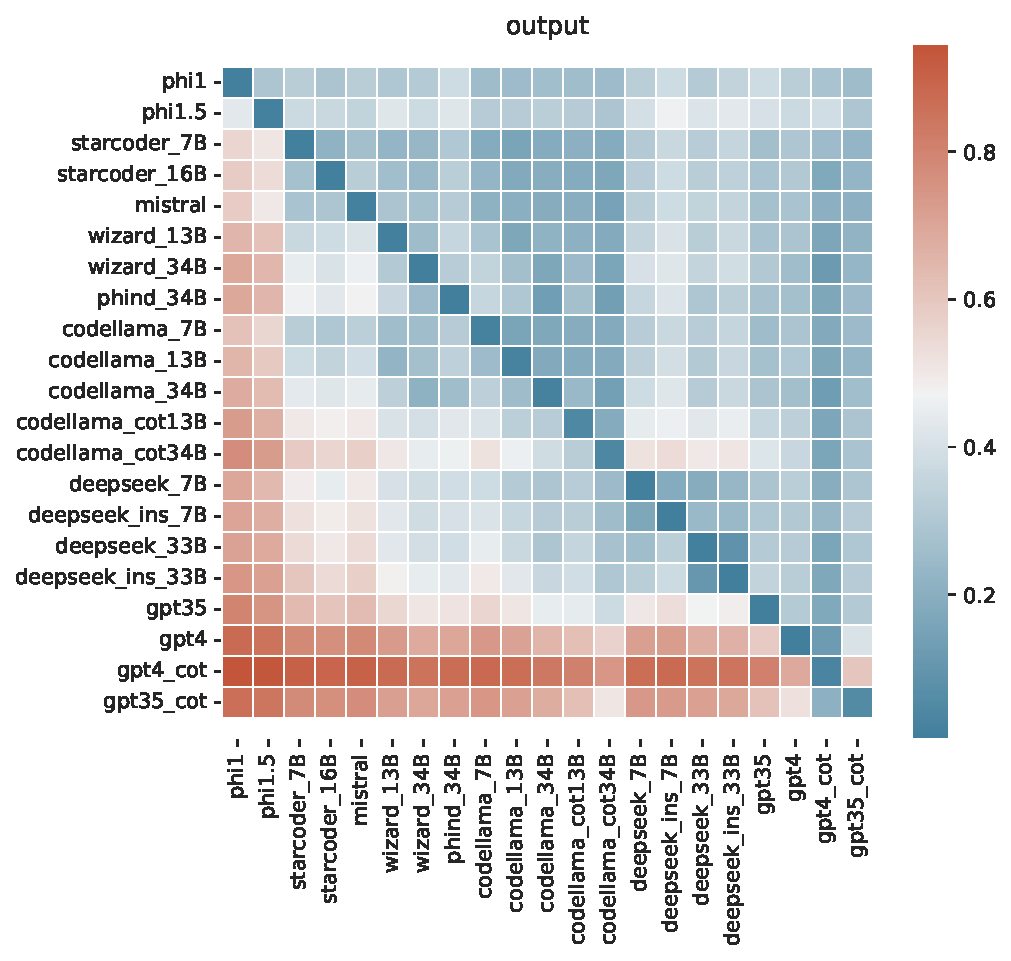
\includegraphics[width=1\textwidth]{figs/error_prob_output_heatmap.pdf}
     \end{subfigure}
     \caption{$P(Y \mid X=0) / P(Y)$ where each $Y$ is the accuracy of models in each row ($X$ for column). }
     \label{fig:error_prob-input-output}
\end{figure}

\subsection{Results on Diversity of Generations} \label{sec:appendix-diversity}

\textbf{Diversity of generations across models}: Next, we analyze the diversity of generated inputs and outputs across various models (without regard to correctness). In Fig. \ref{fig:sample-diversity-direct}, we plot the mean and median number of unique answers generated across samples of \benchmark for a selection of evaluated models. First, we observe the drastic increase in diversity between using $T=0.2$ and $T=0.8$. Second, by comparing Fig. \ref{fig:sample-diversity-direct-input} with Fig. \ref{fig:sample-diversity-direct-output}, we note that input prediction generally has a larger diversity of generations than output prediction. This may be due to the fact that output prediction only has one correct answer, but input prediction may have multiple correct answers. Third, we observe that at the same temperatures, Code Llama models have the highest diversity, while distilled models like Phind and WizardCoder have a lower diversity.


\begin{figure}[H]
     \centering
     \begin{subfigure}[b]{0.49\textwidth}
         \centering
         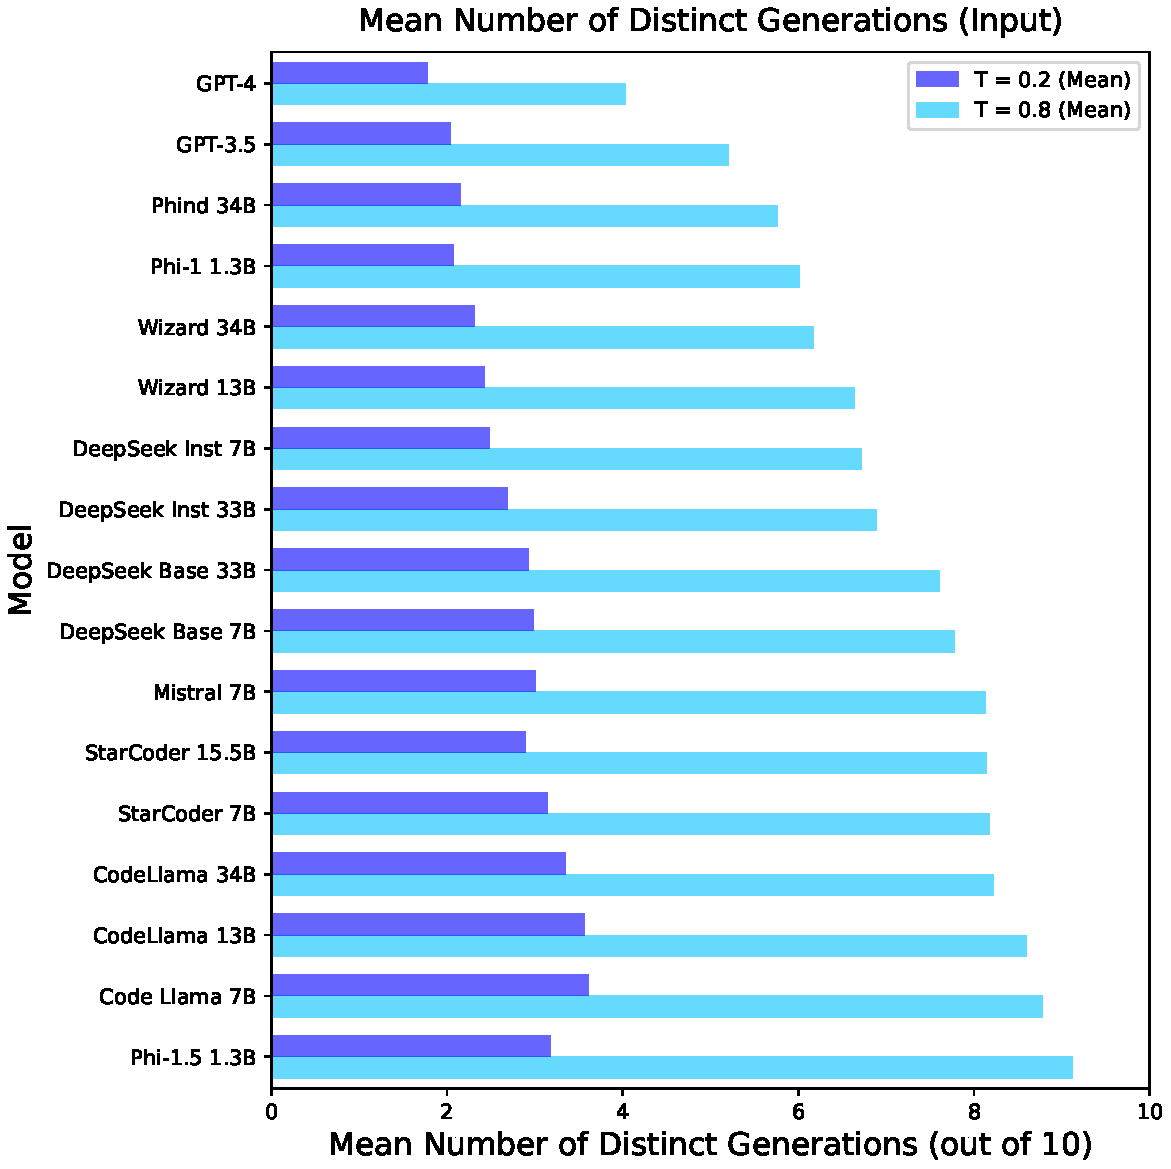
\includegraphics[width=\textwidth]{figs/diversity/diversity_freq_input.pdf}
         \caption{Input prediction}
         \label{fig:sample-diversity-direct-input}
     \end{subfigure}
     \begin{subfigure}[b]{0.49\textwidth}
         \centering
         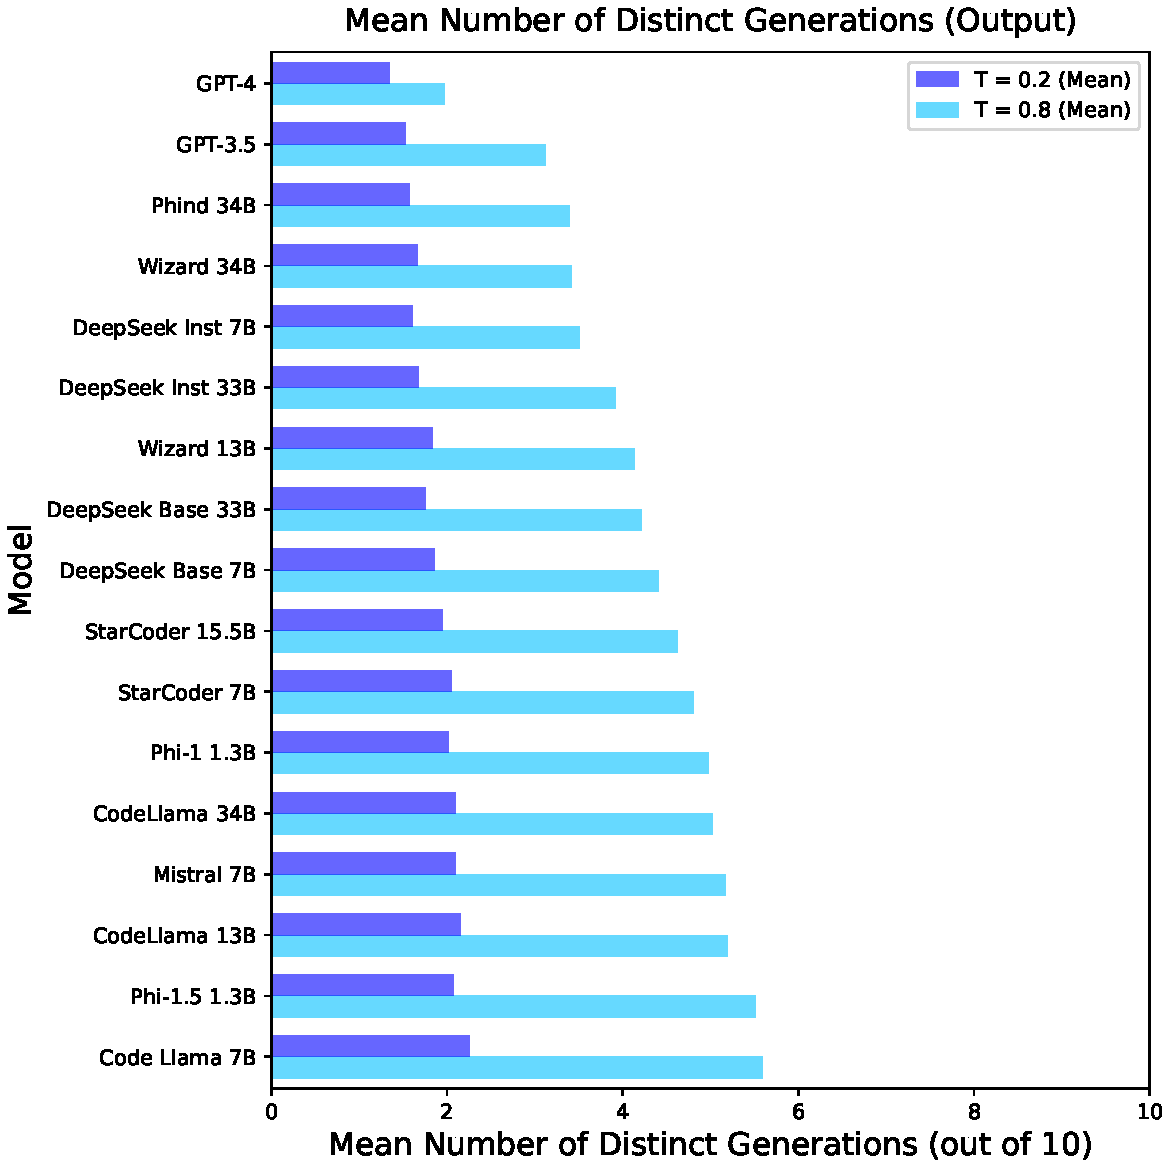
\includegraphics[width=\textwidth]{figs/diversity/diversity_freq_output.pdf}
         \caption{Output prediction}
         \label{fig:sample-diversity-direct-output}
     \end{subfigure}
     \caption{Number of distinct generations of various models (out of 10) at $T=0.2$ and $T=0.8$}
     \label{fig:sample-diversity-direct}
\end{figure}

\textbf{CoT increase the diversity of generations}: In Fig. \ref{fig:sample-diversity-cot}, for each model, we plot the average number of distinct generations across all samples, where different chains of thought with the same input or output prediction are considered identical.  We see again the trend of input prediction generations being more diverse than output prediction generations. Interestingly, we observe that using CoT increases the diversity at both temperatures. 

\begin{figure}[H]
     \centering
     \begin{subfigure}[b]{0.49\textwidth}
         \centering
         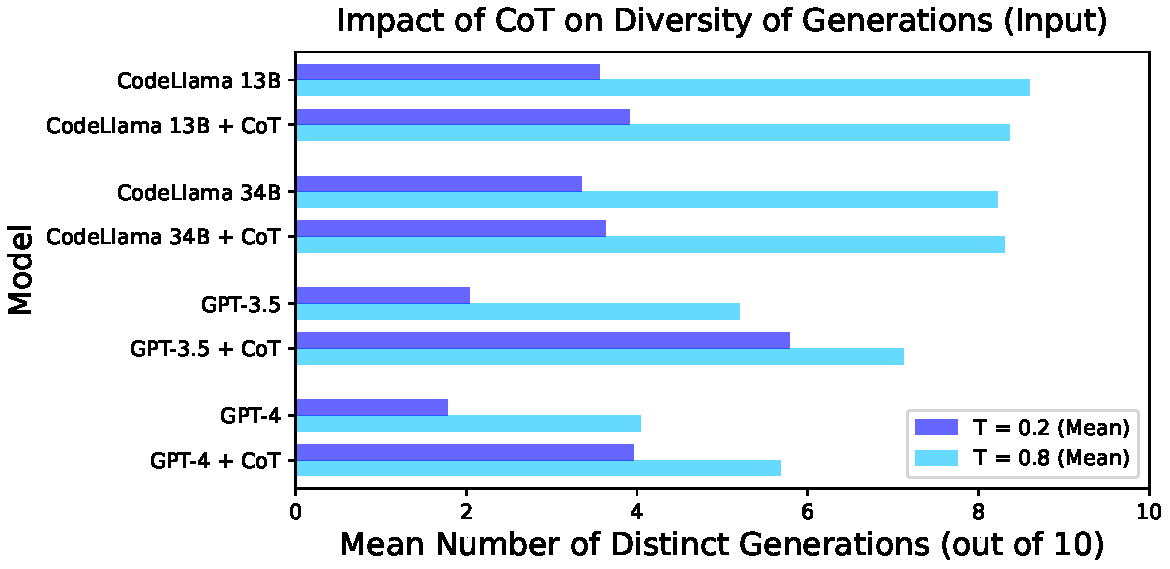
\includegraphics[width=\textwidth]{figs/diversity/diversity_freq_input_cot.pdf}
         \caption{Input prediction}
         \label{fig:sample-diversity-cot-input}
     \end{subfigure}
     \hfill
     \begin{subfigure}[b]{0.49\textwidth}
         \centering
         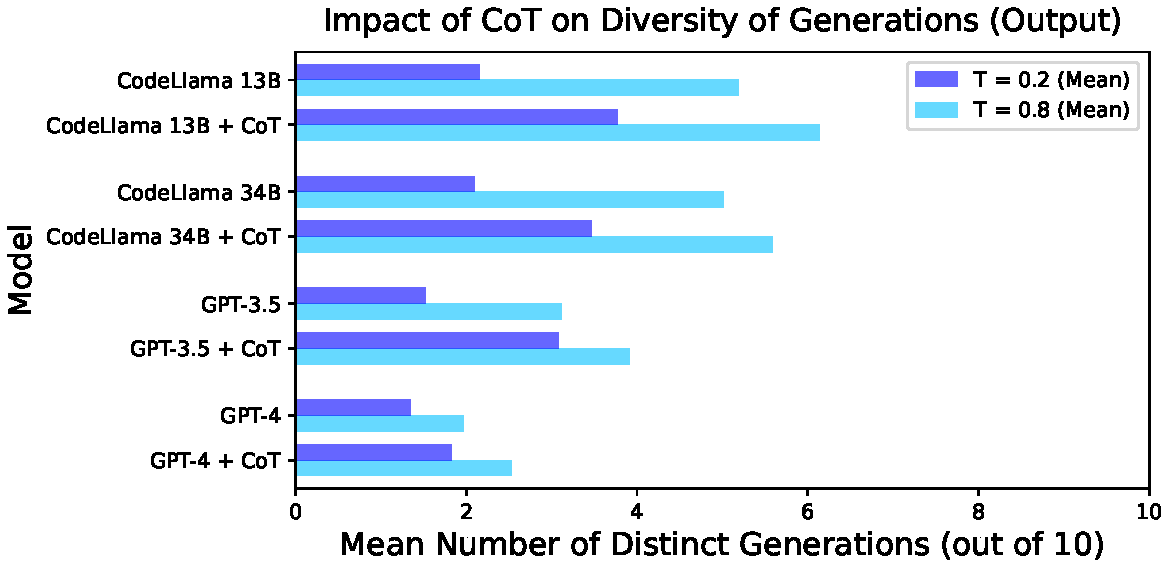
\includegraphics[width=\textwidth]{figs/diversity/diversity_freq_output_cot.pdf}
         \caption{Output prediction}
         \label{fig:sample-diversity-cot-output}
     \end{subfigure}
     \caption{Number of distinct generations of various models (normalized to be out of 10) at $T=0.2$ and $T=0.8$ with and without CoT. We observe that CoT increases the diversity of generations.}
     \label{fig:sample-diversity-cot}
\end{figure}

\textbf{Functional diversity via distribution of pass@1 scores}: In Fig.~\ref{fig:sample-frequency-all}, for each model, we plot the percentage of samples where the pass@1 score $(T=0.2)$ is between $0.1$ and $0.9$, exclusive, indicating that the sample is neither "too easy" nor "too hard" for the model. This is a measure of functional diversity because models with more diversity are likely to generate both correct and incorrect samples, leading to more intermediate pass@1 scores. We make a few observations relatively consistent with our prior observations. First, the percentages are relatively low across the board, indicating that at a temperature of $T=0.2$, models are generally producing a majority of correct or a majority of incorrect outputs. Second, distilled models have a much lower functional diversity than base models, for example comparing Phind 34B to CodeLlama 34B or DeepSeek Instruct 33B to DeepSeek Base 33B. Third, CoT greatly increases the functional diversity of models, which is very evident when looking at GPT-3.5 and GPT-4. 

\begin{figure}[H]
     \centering
     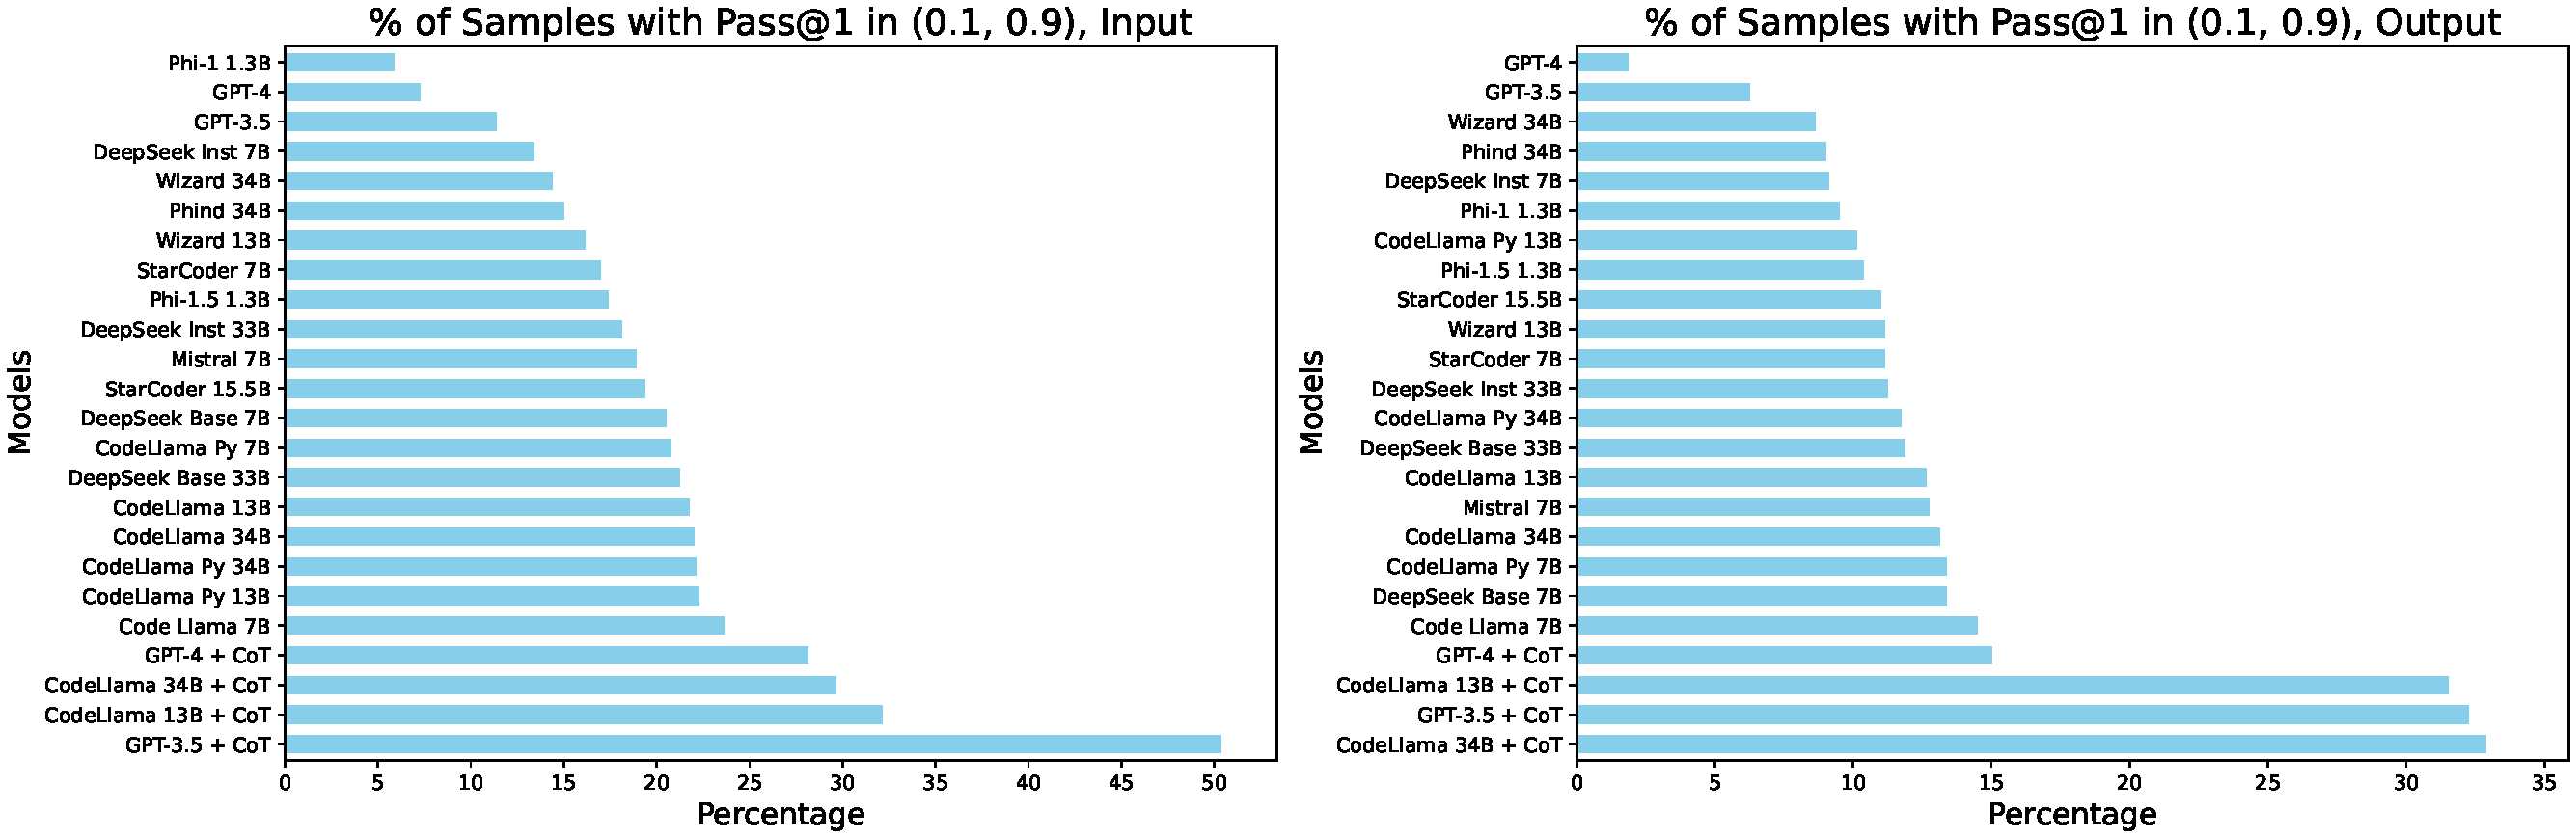
\includegraphics[width=\textwidth]{figs/diversity/frequency_analysis.pdf}
     \caption{Percentage of samples where pass@1 score is in $(0.1, 0.9)$, exclusive.}
     \label{fig:sample-frequency-all}
\end{figure}

\subsection{Difficulty of Benchmark Samples}
\textbf{Distribution of sample difficulties}: In Fig. \ref{fig:benchmark-sample-difficulty}, we show the average pass@1 score across all models for $T=0.2$ in order to get a sense of the difficulty distribution of \benchmark.

\begin{figure}[h]
    \centering
    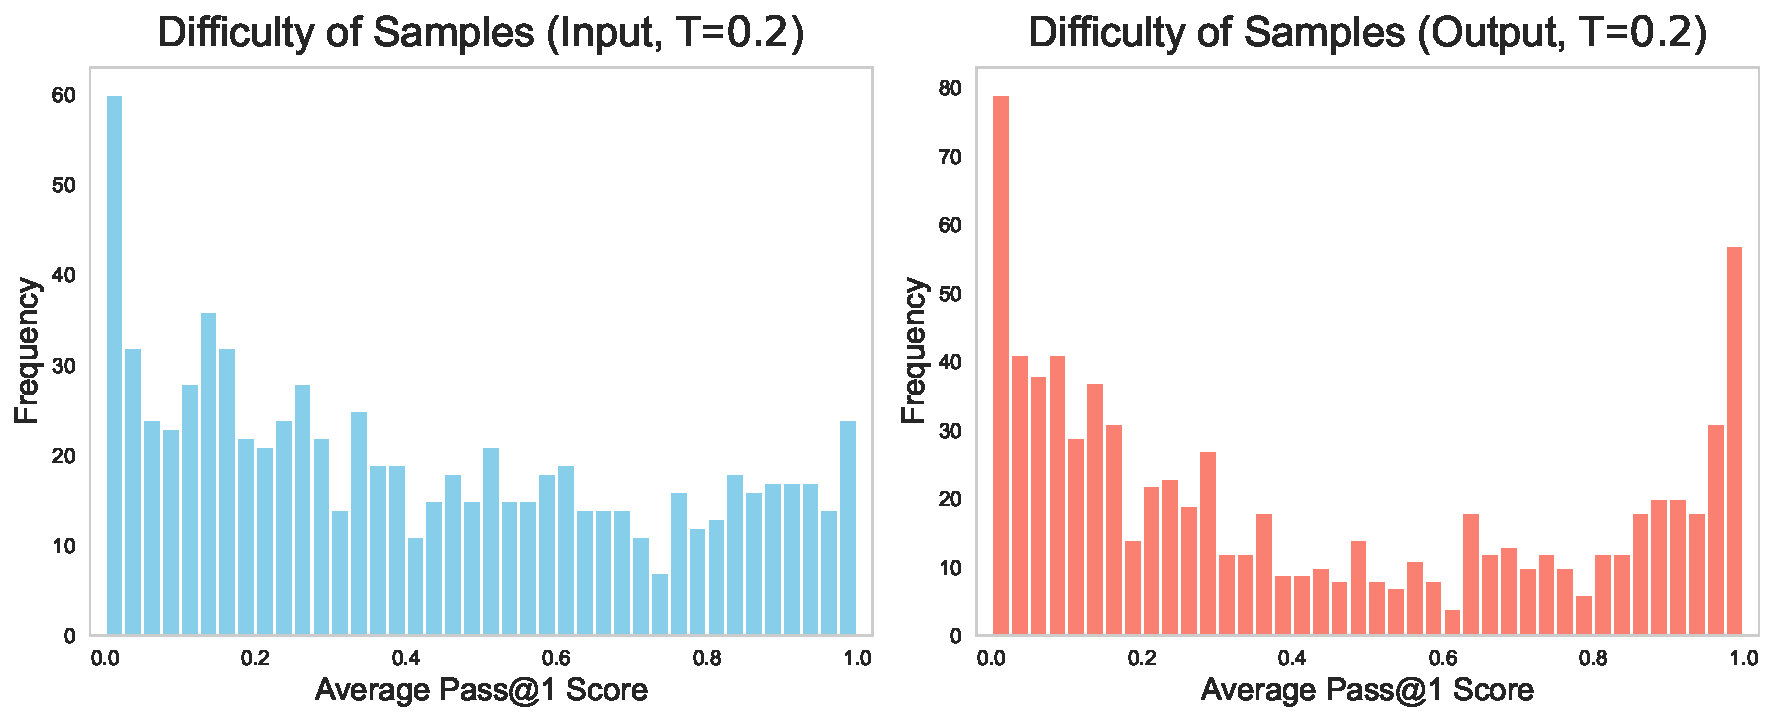
\includegraphics[width=\textwidth]{figs/benchmark/sample_difficulty_0.2.pdf}
    \caption{Difficulty of all samples of our benchmark, averaged across all models $(T=0.2)$}
    \label{fig:benchmark-sample-difficulty}
\end{figure}

In Fig. \ref{fig:pass1-distributions-selected}, we show the pass@1 distributions of a few of the best-performing models at $T=0.8$. Compared to the overall distribution, the distribution appears to be more bimodal. The output prediction distribution is more bimodal than the input prediction distribution, perhaps reflecting the differences in the tasks themselves. We also see the familiar trend of CoT increasing the number of samples with intermediate scores (in this case between $0.25$ and $0.75$).

\begin{figure}[h]
    \centering
     \begin{subfigure}[b]{0.49\textwidth}
         \centering
         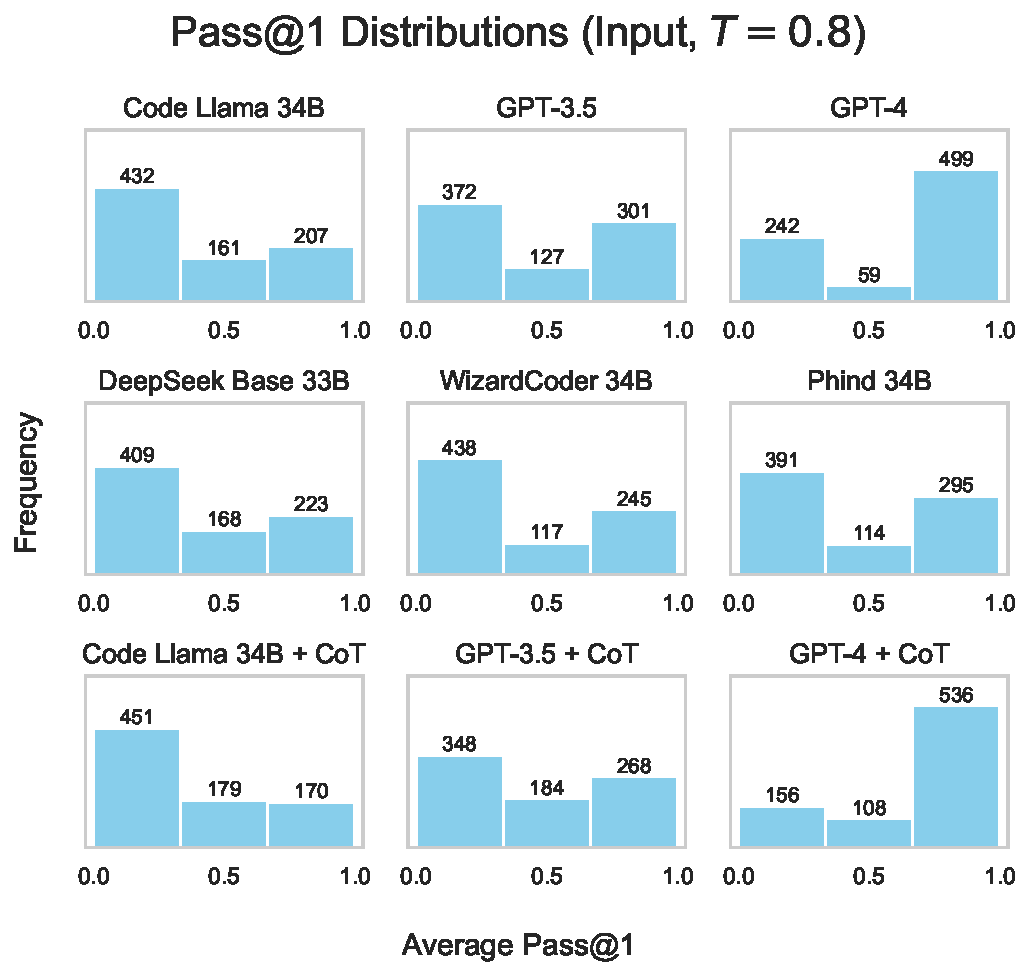
\includegraphics[width=\textwidth]{figs/diversity/sample_pass1_distributions_input_0.8.pdf}
     \end{subfigure}
     \hfill
     \begin{subfigure}[b]{0.49\textwidth}
         \centering
         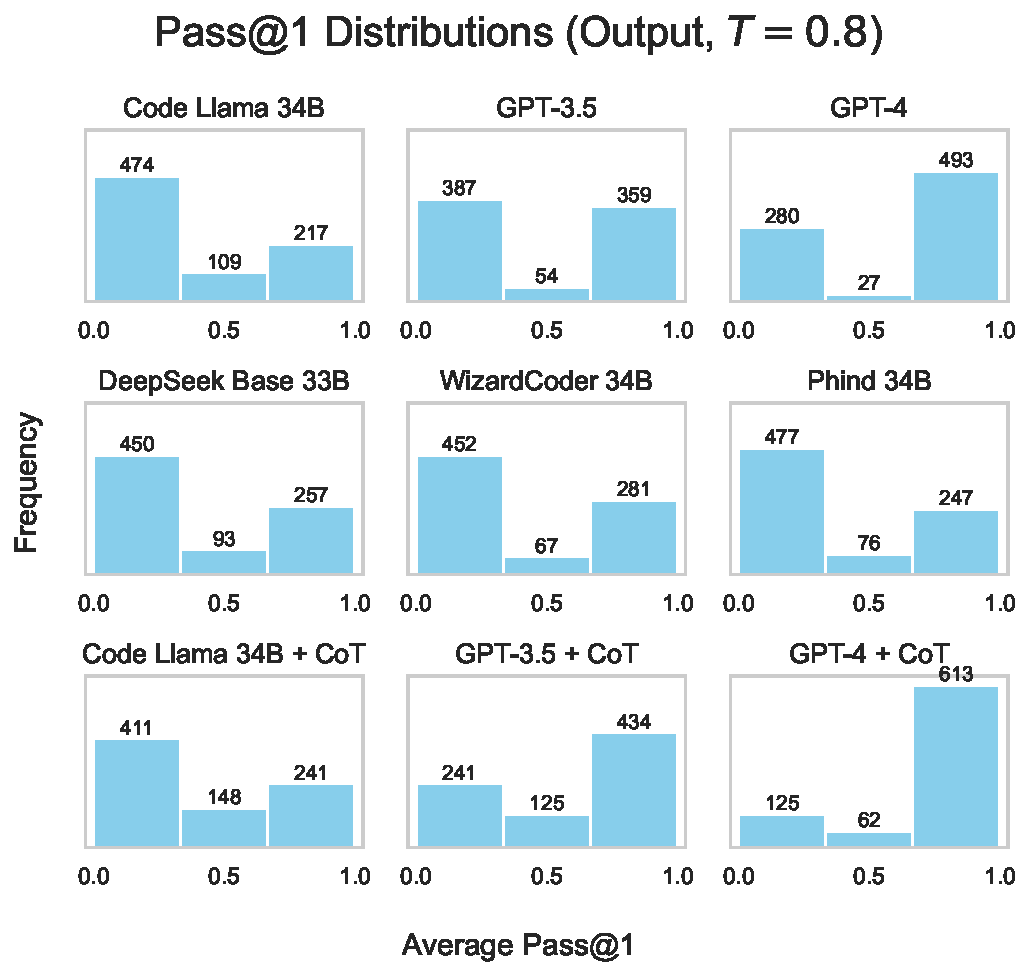
\includegraphics[width=\textwidth]{figs/diversity/sample_pass1_distributions_output_0.8.pdf}
     \end{subfigure}
     \caption{Pass@1 Distributions of Selected Models}
     \label{fig:pass1-distributions-selected}
\end{figure}


\textbf{Fully solved and unsolved samples}: In Figs. \ref{fig:sample-frequency-unsolved} and \ref{fig:sample-frequency-fully-solved}, we examine a different metric, the percentage of examples with pass@1 score equal to $0$ and $1$, respectively, at $T=0.8$. In a sense, this metric captures the ability of models to solve problems. It is also related to diversity, as with a higher diversity, the likelihood of solving the problem may increase. A few observations arise from looking at this metric.

Fig. \ref{fig:sample-frequency-unsolved}, shows the percentage of samples that are completely unsolved by each model, i.e. with $0$ pass@1. We analyze this metric for $T=0.8$, because it leads to more diversity, which would improve this metric. First, when considering non-CoT modes, while GPT-3.5 and GPT-4 (red) are the two best-performing models at pass@1, they perform considerably worse at this metric than models such as Code Llama 34B and DeepSeek Base 33B. Second, instruction-tuned and distilled models (DeepSeek Instruct, Phind, WizardCoder) perform worse than their base counterparts, suggesting that their diversity may have been stifled from adherence to their instruction tuning datasets. Third, we observe that for the two Code Llama models, CoT actually makes this metric worse, but for GPT models, CoT makes it better. For GPT models, we hypothesize that this may be due to the increased diversity of CoT. 

\begin{figure}[H]
     \centering
     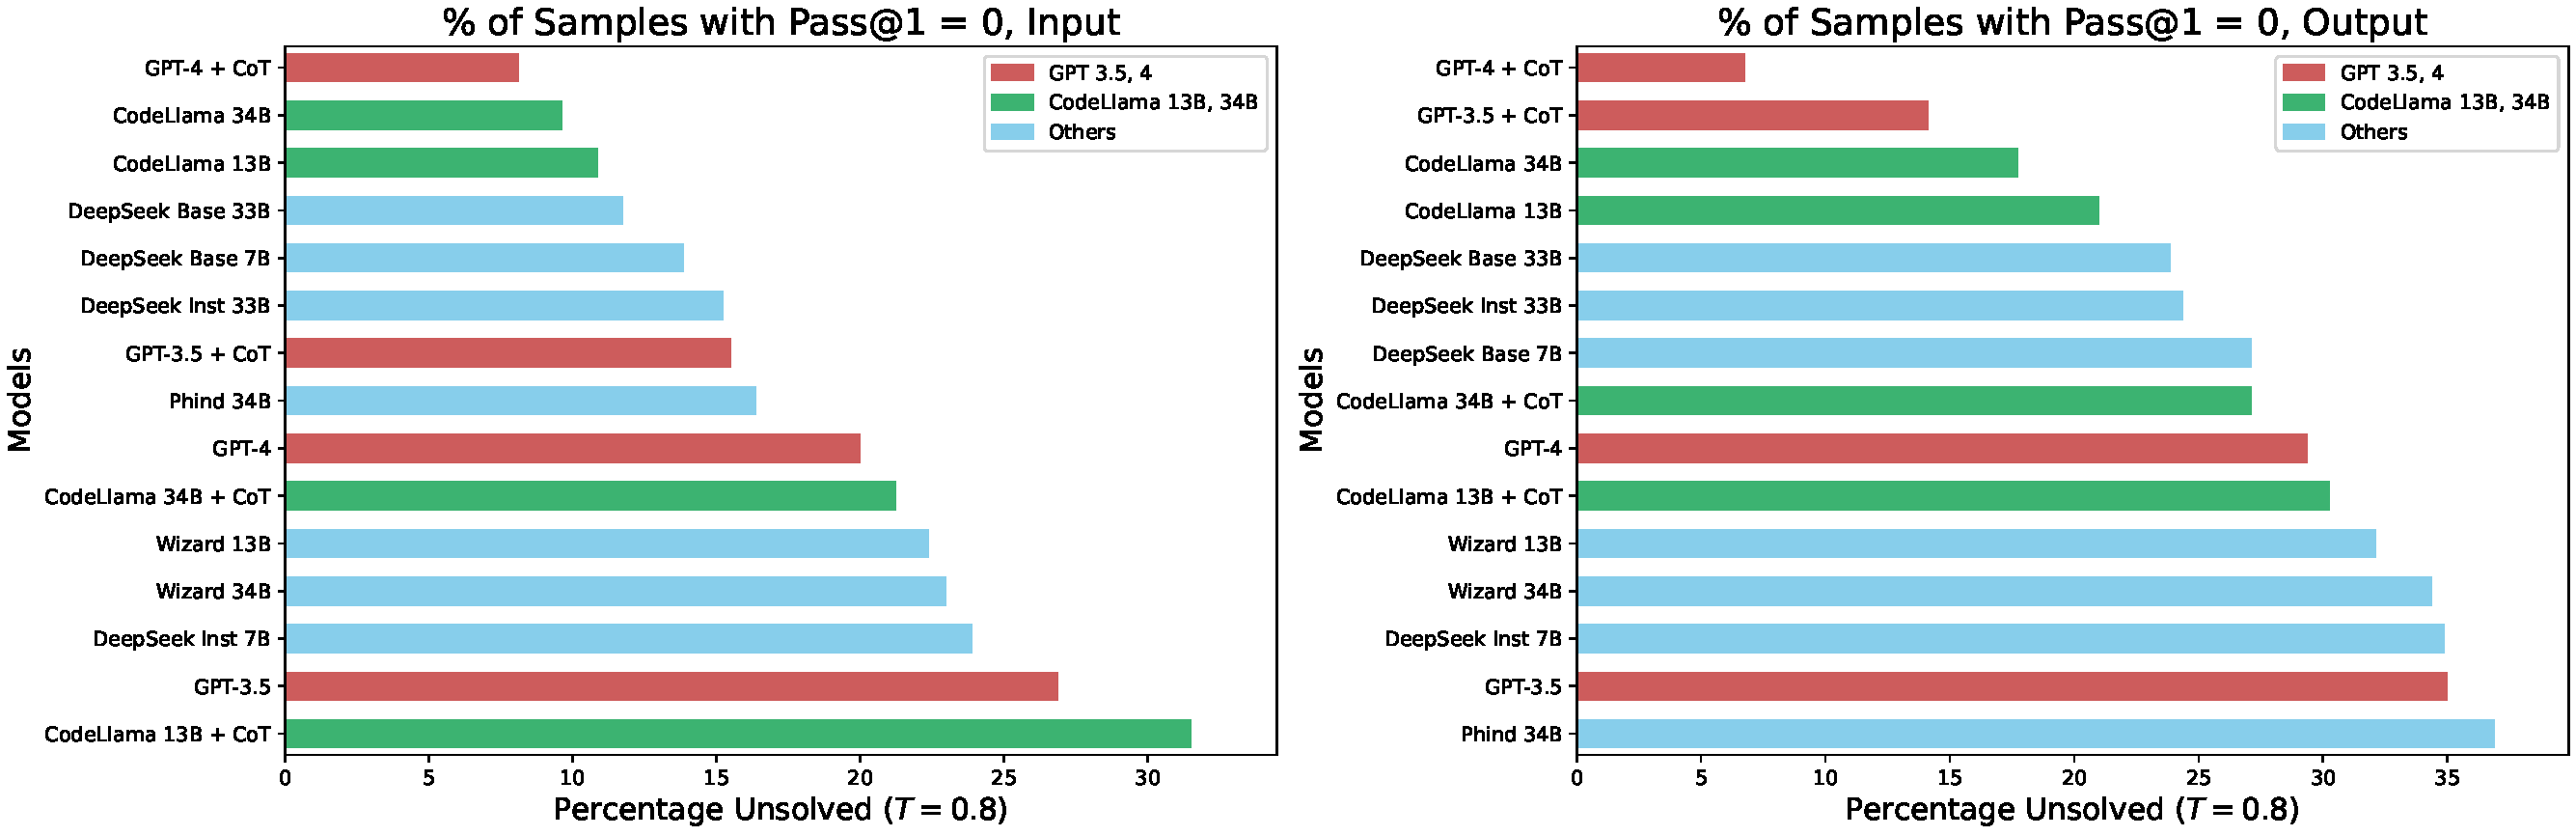
\includegraphics[width=\textwidth]{figs/diversity/unsolved_analysis_0.8.pdf}
     \caption{Percentage of samples unsolved, where pass@1 is $0$ ($T=0.8$)}
     \label{fig:sample-frequency-unsolved}
\end{figure}

In contrast, Fig. \ref{fig:sample-frequency-fully-solved} shows the percentage of samples that models get fully correct, i.e. with a perfect pass@1. We analyze this metric for $T=0.2$, as it would lead to more consistency, improving this metric. First, we see that GPT-4 excels, achieving over 60\% for both input and output prediction. Second, when comparing base models with instruction tuned models, we see a trend matching the one before: since instruction tuned models are more consistent, they score better on this metric. Third, for output prediction, even though GPT-4 + CoT generally increases diversity, we see that consistency is not sacrificed!

\begin{figure}[H]
     \centering
     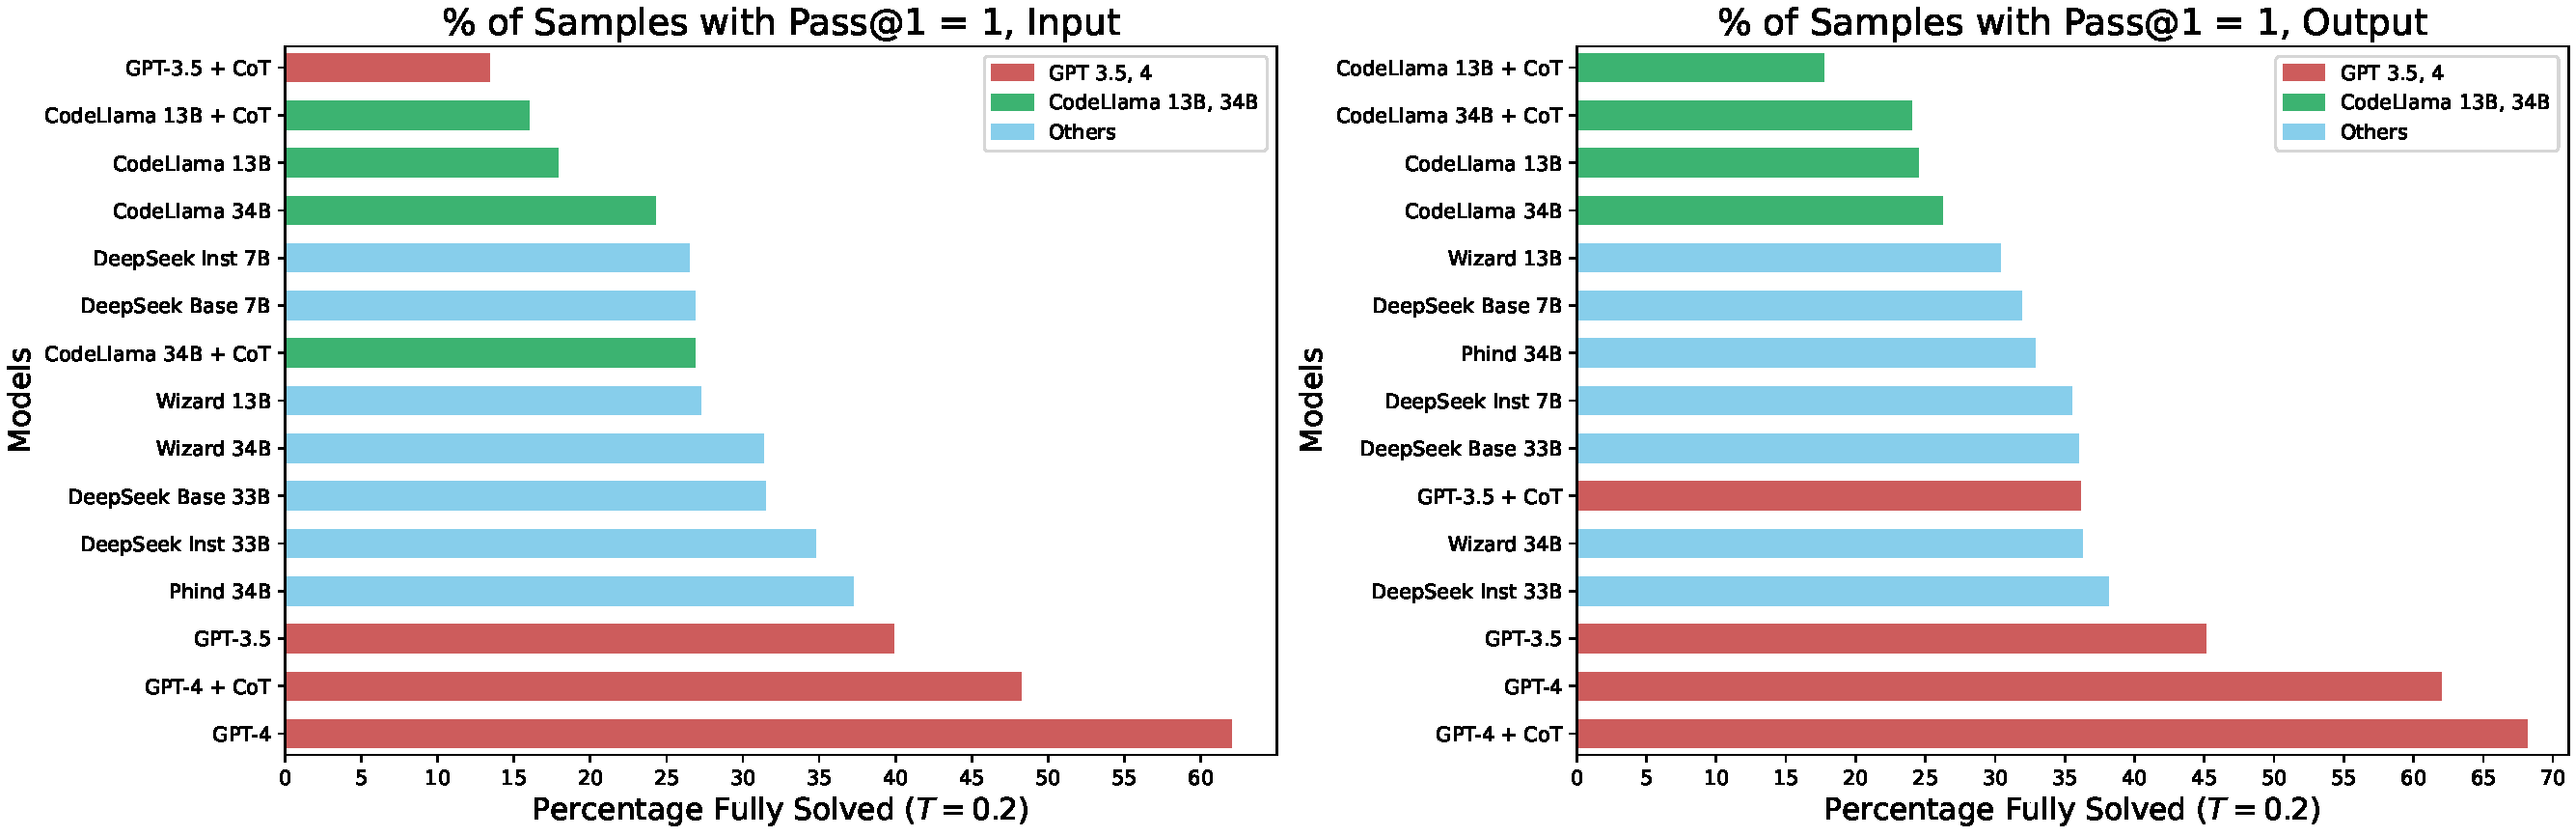
\includegraphics[width=\textwidth]{figs/diversity/fully_solved_analysis_0.2.pdf}
     \caption{Percentage of samples fully solved, where pass@1 score is $1$ ($T=0.2$)}
     
     \label{fig:sample-frequency-fully-solved}
\end{figure}


\subsection{Impact of Anonymizing Functions} \label{sec:appendix-anonymization}
As a small ablation to understand the effect of variable names on execution ability, we also test CodeLlama 7B, 13B, and 34B on an anonymized version of a subset of the benchmark, where variable names are replaced with \texttt{x1, x2, ...} identifiers. An example of an anonymized function is shown in Listing \ref{lst:benchmark-anonymized-sample}. We use the same few-shot prompt without anonymization and report both pass@1 ($T=0.2$) and pass@5 ($T=0.8$) results on the anonymized benchmark with $N=10$ samples. The results are shown in Table \ref{tab:benchmark-results-anonymous}. This strengthens the case against memorization affects.

\begin{lstlisting}[caption={Sample of benchmark and anonymized version},label={lst:benchmark-anonymized-sample}, captionpos=t, breaklines=true]
Original:
def f(s):
    nums = ''.join(filter(lambda c:c.isdecimal(), s))
    if nums == '': return 'none'
    m = max([int(num) for num in nums.split(',')])
    return str(m)
assert f('01,001') == '1001'

Anonymized:
def f(x0):
    x1 = ''.join(filter(lambda x2: x2.isdecimal(), x0))
    if x1 == '':
        return 'none'
    x3 = max([int(x4) for x4 in x1.split(',')])
    return str(x3)
assert f('01,001') == '1001'
\end{lstlisting}

\begin{table}[htbp]
    \centering
    \caption{Impact of Anonymization on \benchmark}
    \begin{tabular}{cccccc}
        \toprule
        \multirow{2}{*}{\textbf{Model}} & \multirow{2}{*}{\textbf{Anonymized}} & \multicolumn{2}{c}{\textbf{Input Prediction}} & \multicolumn{2}{c}{\textbf{Output Prediction}} \\
        \cmidrule(lr){3-4} \cmidrule(lr){5-6}
        & & \textbf{Pass@1} & \textbf{Pass@5} & \textbf{Pass@1} & \textbf{Pass@5} \\
        \midrule
        \multirow{3}{*}{CodeLlama 7B} 
	& \xmark & 36.6\% & 48.0\% & 36.4\% & 43.5\% \\
        & \cmark & 37.5\% & 53.3\% & 34.0\% & 46.9\% \\
        & $\Delta$ & \green{+0.9\%} & \green{+5.3\%} & \red{-2.4\%} & \green{+3.4\%} \\
        \midrule
        \multirow{3}{*}{CodeLlama 13B} 
        & \xmark & 39.0\% & 50.2\% & 38.3\% & 44.7\% \\
        & \cmark & 40.0\% & 55.8\% & 36.1\% & 50.6\% \\
        & $\Delta$ & \green{+1.0\%} & \green{+5.6\%} & \red{-2.2\%} & \green{+5.9\%} \\
        \midrule
        \multirow{3}{*}{CodeLlama 34B} 
        & \xmark & 46.5\% & 57.4\% & 41.1\% & 47.5\% \\
        & \cmark & 48.0\% & 63.8\% & 39.1\% & 54.0\% \\
        & $\Delta$ & \green{+1.5\%} & \green{+6.4\%} & \red{-2.0\%} & \green{+6.5\%} \\
        \bottomrule
    \end{tabular}
    \label{tab:benchmark-results-anonymous}
\end{table}

\subsection{Impact of Data-Generating Model}
In the early phases of this work, we were concerned that using Code Llama 34B to generate the benchmark would give the model an unfair advantage. Therefore, we checked the performance of a few models when generating data with Code Llama 13B, GPT-3.5, and GPT-4. The results are shown in Table \ref{tab:benchmark-results-data-generating}. 

These samples were generated using a different prompt and a much more relaxed filter, so the raw scores differ from those in the main text. Across all datasets, we see that the relative ordering of Code Llama 13B, Code Llama 34B, and GPT-3.5 are preserved. We also observed that generating data with GPT-3.5 led to a significantly easier benchmark. After looking at a few samples manually, we believe this is because the resulting inputs are much more predictable and guessable, such as \texttt{f("abcde")} rather than \texttt{f("mai2!")}. Including few-shot examples with random inputs did not improve this issue, and we believe this is an artifact of instruction tuning. We believe that together with the anonymization results in Appendix \ref{sec:appendix-anonymization}, these results provide some evidence that evaluating a model on its own generated data does not seem to provide it a significant advantage.


\begin{table}[H]
    \centering
    \caption{Impact of Data Generating Model}
    \begin{tabular}{cccc}
        \toprule
        \textbf{Data Model} & \textbf{Evaluation Model} & \textbf{Input Pass@1} & \textbf{Output Pass@1} \\
        \midrule
        CL 13B & CL 13B & 28.1\% & 28.4\% \\
        CL 13B & CL 34B & 33.8\% & 29.2\% \\
        \midrule
        CL 34B & CL 13B & 25.1\% & 24.3\% \\
        CL 34B & CL 34B & 29.9\% & 25.4\% \\
        CL 34B & GPT-3.5 & 40.5\% & 36.6\% \\
        \midrule
        GPT-3.5 & CL 13B & 42.3\% & 49.7\% \\
        GPT-3.5 & CL 34B & 52.1\% & 50.7\% \\
        GPT-3.5 & GPT-3.5 & 67.1\% & 67.2\% \\
        \midrule
        GPT-4 & CL 13B & 28.1\% & 42.4\% \\
        GPT-4 & CL 34B & 37.0\% & 44.6\% \\
        \bottomrule
    \end{tabular}
    \label{tab:benchmark-results-data-generating}
\end{table}

\subsection{Fine-tuning} \label{subsec:appendix-finetuning}
We discover three interesting insights from fine-tuning. In the main text, we only discuss insight 3. As a refresher, we fine-tuned \codellamalarge on 138889 samples of Python functions distilled with the procedure outlined in Sec. \ref{sec:benchmark-construction}, without filtering. For the output prediction task, the model was fine-tuned on assertions of the form \texttt{assert f(input) == output}, and for the input prediction task, the model was fine-tuned on assertions of the form \texttt{assert output == f(input)}. During evaluation time, the fine-tuned model was asked to complete assertions of the same format as given in fine-tuning. 

\textbf{1. Direct fine-tuning leads to modest performance improvements}: In the first setup, we analyze a stronger decontamination setup than that in the main text. Specifically, we remove samples that match functions used in the benchmark, even if the input-output pairs are different. In Fig. \ref{fig:finetuning-accuracy-plot}, we show the train and test accuracy of the model during the finetuning process. For ease of evaluation, the train accuracy is reported on a random subset of 500 samples from the finetuning set. The reported test accuracy is on a superset of \benchmark. 

First, we observe that fine-tuning is able to significantly increase performance on both input and output prediction tasks. Second, we observe that while the training accuracy is steadily increasing and the model is able to overfit the training set, the testing accuracy plateaus relatively quickly. This suggesting that simple fine-tuning may not be enough to achieve near-perfect scores on \benchmark. Third, we observe that it is easier to overfit the training set on the output prediction benchmark than on the input prediction benchmark. We hypothesize this may be partially due to the fact that \texttt{assert output == f(input)} is a less natural format for assertions and partially due to the fact that input prediction requires a more sophisticated level of reasoning compared to output prediction.

\begin{figure}[H]
     \centering
     \begin{subfigure}[b]{0.48\textwidth}
         \centering
         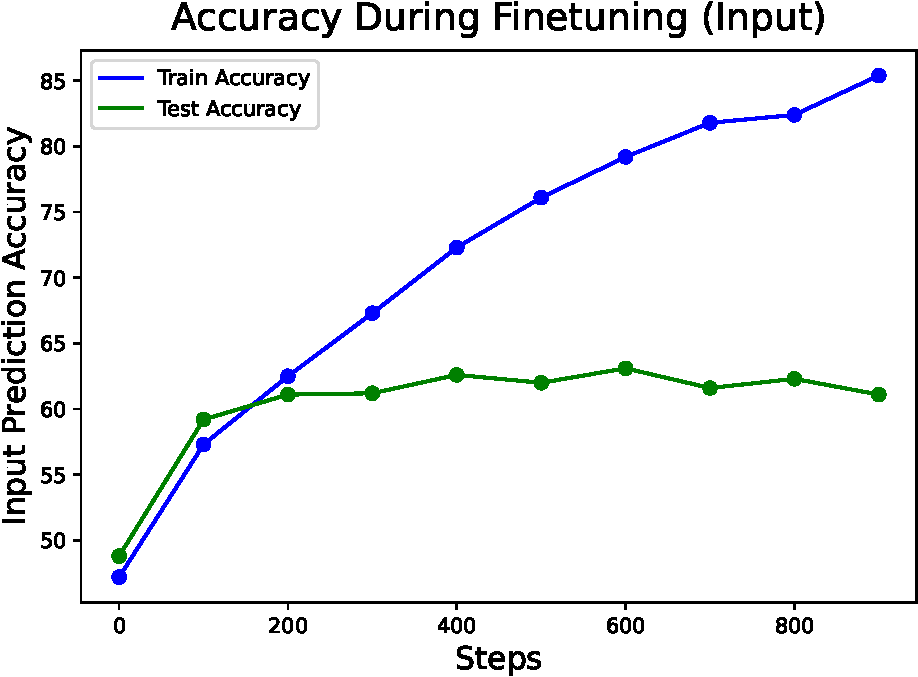
\includegraphics[scale=0.4]{figs/finetuning/finetuning_input_accuracy.pdf}
         \caption{Input prediction}
         \label{fig:finetuning-accuracy-plot-input}
     \end{subfigure}
     \hfill
     \begin{subfigure}[b]{0.48\textwidth}
         \centering
         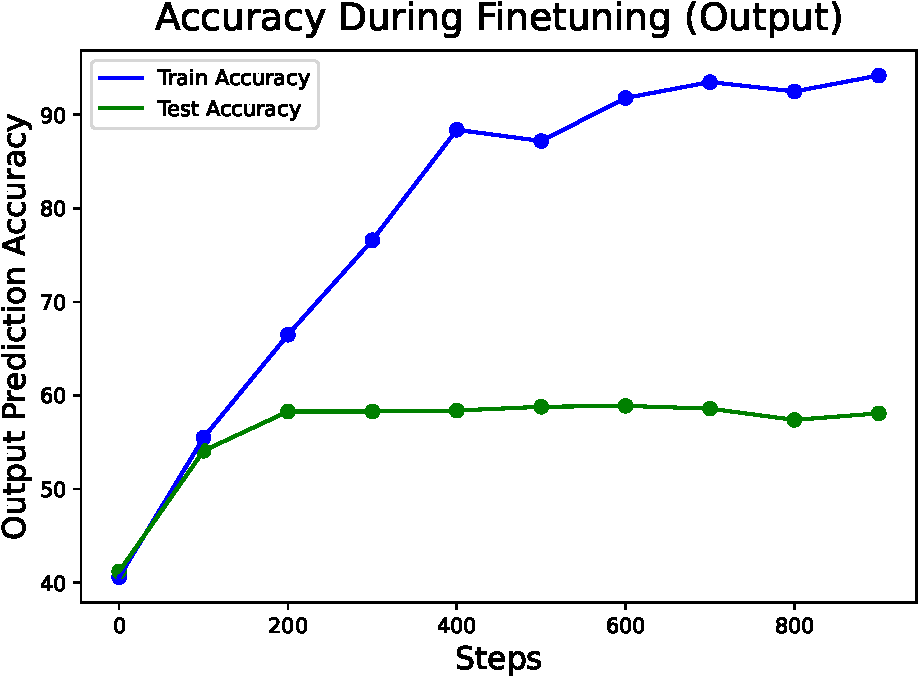
\includegraphics[scale=0.4]{figs/finetuning/finetuning_output_accuracy.pdf}
         \caption{Output prediction}
         \label{fig:finetuning-accuracy-plot-output}
     \end{subfigure}
     \caption{Train accuracy (500 random samples) and test accuracy (superset of \benchmark) while finetuning. For both tasks, there is improvement, and the model steadily fits the training set while plateauing on the testing set.}
     \label{fig:finetuning-accuracy-plot}
\end{figure}

\textbf{2. The format of fine-tuning data greatly impacts its effectiveness}: We also discovered that it is important that the finetuning assertions be formatted in the same way as when evaluating the model at test time. As evidence of this, we fine-tune \codellamalarge with two different sets of assertions, one on \texttt{assert output == f(input)} assertions and the other on \texttt{assert f(input) == output} assertions. We compare the accuracy of the two finetuned models on both input and output prediction in Fig. \ref{fig:finetuning-accuracy-format-plot}. We observe that when the format of the fine-tuning data and the testing data are different, the model even has difficulty overfitting the training set, showing that it may not have fully learned the equivalence of the two formats and the meaning of the \texttt{==} operator. This is perhaps another example of the ``reversal curse'' of LLMs \citep{berglund2023reversal}. The corresponding testing accuracy also plateaued at a lower accuracy when the format was misaligned. For example, in Fig. \ref{fig:finetuning-accuracy-format-plot-input}, comparing the light green line with the light blue line shows almost a 10\% difference in testing accuracy for input prediction when trained on a misaligned format. That being said, fine-tuning still improved performance relative to the base model, even with a mismatched format, showing that the fine-tuning with a mismatched format did still instill some information into the model.

\begin{figure}[H]
     \centering
     \begin{subfigure}[b]{0.48\textwidth}
         \centering
         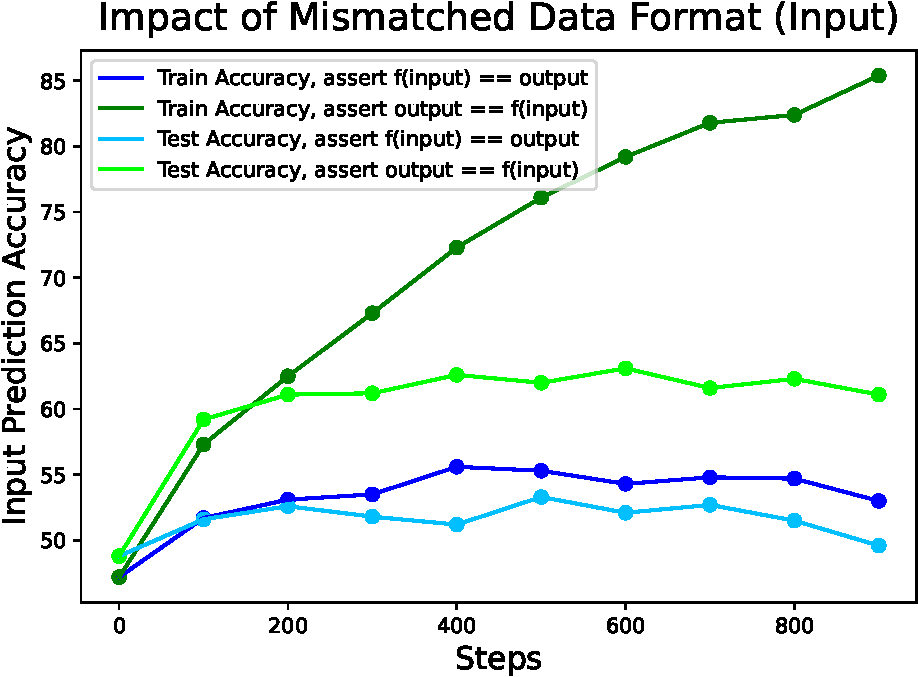
\includegraphics[scale=0.4]{figs/finetuning/finetuning_input_format.pdf}
         \caption{Input prediction}
         \label{fig:finetuning-accuracy-format-plot-input}
     \end{subfigure}
     \hfill
     \begin{subfigure}[b]{0.48\textwidth}
         \centering
         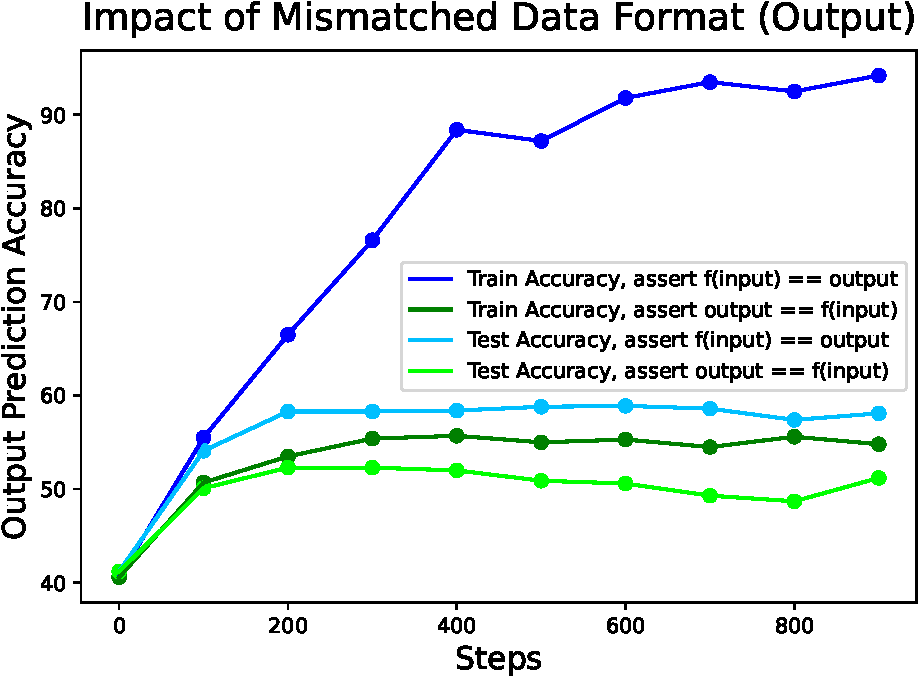
\includegraphics[scale=0.4]{figs/finetuning/finetuning_output_format.pdf}
         \caption{Output prediction}
         \label{fig:finetuning-accuracy-format-plot-output}
     \end{subfigure}
     \caption{Aligning the fine-tuning data format with the evaluation data format is very important for benchmark performance.}
     \label{fig:finetuning-accuracy-format-plot}
\end{figure}

\textbf{3. Including benchmark programs still cannot improve test accuracy beyond 70\%}: Finally, we explore the upper limits of fine-tuning on functions and assertions via a "cheating" setup. We curate a small set of \textit{7259 samples consisting only of programs in the benchmark} but with different input-output pairs. We finetune on a mixture of 50\% of the original finetuning set and 50\% of this new set, showing the training and testing accuracy over time in Fig. \ref{fig:finetuning-accuracy-samples-plot}. Despite finetuning on programs very similar to the benchmark, we still observe a plateauing effect in the test accuracy, suggesting that our execution tasks may be too difficult to learn from this simple fine-tuning scheme. Therefore, we suggest a few more fine-tuning ideas for improving our benchmark in Sec. \ref{sec:limitations-future-work}.

% \begin{figure}
%      \centering
%      \begin{subfigure}[b]{0.48\textwidth}
%          \centering
%          \includegraphics[scale=0.4]{figs/finetuning/finetuning_input_samples.pdf}
%          \caption{Input prediction}
%          \label{fig:plots:a}
%      \end{subfigure}
%      \hfill
%      \begin{subfigure}[b]{0.48\textwidth}
%          \centering
%          \includegraphics[scale=0.4]{figs/finetuning/finetuning_output_samples.pdf}
%          \caption{Output prediction}
%          \label{fig:plots:b}
%      \end{subfigure}
%      \caption{Including programs from the benchmark dataset leads to a small boost.}
%      \label{fig:finetuning-accuracy-samples-plot}
% \end{figure}

\begin{figure}[H]
     \centering
     \begin{subfigure}[b]{0.48\textwidth}
         \centering
         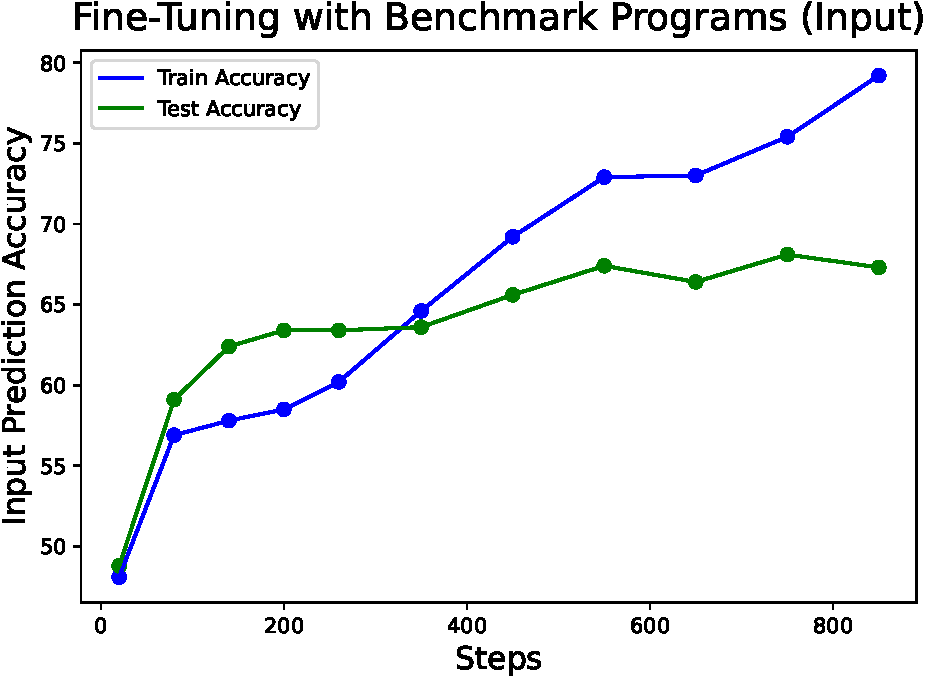
\includegraphics[scale=0.4]{figs/finetuning/finetuning_input_moredata_accuracy.pdf}
         \caption{Input prediction}
         \label{fig:finetuning-accuracy-samples-plot-input}
     \end{subfigure}
     \hfill
     \begin{subfigure}[b]{0.48\textwidth}
         \centering
         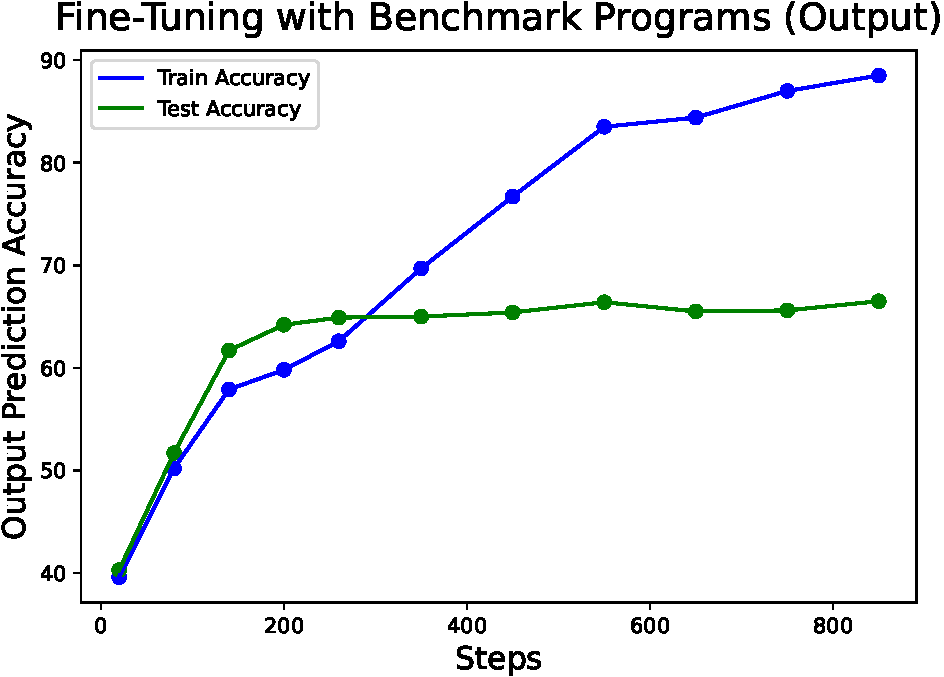
\includegraphics[scale=0.4]{figs/finetuning/finetuning_output_moredata_accuracy.pdf}
         \caption{Output prediction}
         \label{fig:finetuning-accuracy-samples-plot-output}
     \end{subfigure}
     \caption{Finetuning 50\% on the original finetuning set and 50\% on "cheating" data}
     \label{fig:finetuning-accuracy-samples-plot}
\end{figure}